\documentclass[11pt,a4paper]{article}
\usepackage{amssymb}
\usepackage[margin=1in]{geometry}
\usepackage[
backend=biber,
style=science,
]{biblatex}
\usepackage{graphicx}
\usepackage{booktabs}
\usepackage[mathlines]{lineno}
\usepackage{xr}
\usepackage{todonotes}

\usepackage{xcolor}
\usepackage{longtable}
% package to open file containing variables
\usepackage{datatool, filecontents}
\usepackage[scaled]{helvet}
\renewcommand\familydefault{\sfdefault} 

\usepackage{mathastext}

\usepackage[T1]{fontenc}
\usepackage{caption}
\captionsetup[figure]{font=small}
\captionsetup[table]{font=small}
\newcommand{\beginsupplement}{%
    \setcounter{figure}{0}%
    \renewcommand{\thefigure}{S\arabic{figure}}%
    \setcounter{table}{0}%
    \renewcommand{\thetable}{S\arabic{table}}%
}

\usepackage{float}
\usepackage{pdflscape} 

\DTLsetseparator{,}% Set the separator between the columns.

% import data
\DTLloaddb[noheader, keys={thekey,thevalue}]{sc_latency}{../results/beast/processed/sc.latency.csv}
\newcommand{\scLatency}[1]{\DTLfetch{sc_latency}{thekey}{#1}{thevalue}}

\DTLloaddb[noheader, keys={thekey,thevalue}]{sc_latency_noMakona}{../results/beast/processed/sc.latency.noMakona.csv}
\newcommand{\scLatencyNoMakona}[1]{\DTLfetch{sc_latency_noMakona}{thekey}{#1}{thevalue}}

\DTLloaddb[noheader, keys={thekey,thevalue}]{sc_latency_noMakona_noKasai}{../results/beast/processed/sc.latency.noMakona.18.csv}
\newcommand{\scLatencyNoMakonaNoKasai}[1]{\DTLfetch{sc_latency_noMakona_noKasai}{thekey}{#1}{thevalue}}


\DTLloaddb[noheader, keys={thekey,thevalue}]{expectations_noMakona}{./figures/futureFigure.withKasai.csv}
\newcommand{\expectations}[1]{\DTLfetch{expectations_noMakona}{thekey}{#1}{thevalue}}

% also no makona
\DTLloaddb[noheader, keys={thekey,thevalue}]{expectations_noKasai}{./figures/futureFigure.csv}
\newcommand{\expectationsNoKasai}[1]{\DTLfetch{expectations_noKasai}{thekey}{#1}{thevalue}}

\DTLloaddb[noheader, keys={thekey,thevalue}]{ml}{./figures/rtt.csv}
\newcommand{\ml}[1]{\DTLfetch{ml}{thekey}{#1}{thevalue}}

\DeclareUnicodeCharacter{2212}{\ensuremath{-}}

\addbibresource{refs.bib} 


\title{Evidence of latency reshapes our understanding of Ebola virus reservoir dynamics}
%  TODO fix affiliation order once list is finalized
 \author{
     John T.~McCrone$^{1}$
     \and
     Guy Baele$^2$
     \and
     Ifeanyi F.~Omah$^3$
     \and
     Eddy Kinganda-Lusamaki$^{4,5}$
     \and
     Joseph A.~Brew$^{6}$
     \and
     Luiz M.~Carvalho$^7$
     \and
     Nicola F.~M\"uller$^8$
     \and
     Gytis Dudas$^9$
     \and
     Placide Mbala-Kingebeni$^{4,10}$
     \and
     Marc A.~Suchard$^{11,12,13}$
     \and
     Andrew Rambaut$^3$
}
\date{%
\footnotesize
    $^1$Vaccine and Infectious Disease Division, Fred Hutchinson Cancer Center, Seattle, Washington, USA\\
    $^2$Department of Microbiology, Immunology and Transplantation, Rega Institute, KU Leuven, Leuven, Belgium\\
    $^3$Institute of Ecology and Evolution, University of Edinburgh, Edinburgh, UK\\
    $^4$Institut National de Recherché Biomedicale, University of Kinshasa, Kinshasa, Democratic Republic of the Congo\\
    $^5$TransVIHMI, Université de Montpellier, Montpellier, France\\
    $^{6}$ Department of Biomedical Informatics, Harvard Medical School, Boston, MA, USA \\
    $^7$School of Applied Mathematics, Getulio Vargas Foundation (FGV), Rio de Janeiro, Brazil\\
    $^8$Division of HIV, Infectious Diseases, and Global Medicine, University of California, San Francisco, San Francisco,
California, United States\\
    $^9$Institute of Biotechnology, Life Sciences Centre, Vilnius University, Vilnius, Lithuania\\
    $^{10}$South African National Bioinformatics Institute, University of the Western Cape, South Africa\\
    $^{11}$Department of Biostatistics, Fielding School of Public Health, University of California, Los Angeles, CA, USA\\
    $^{12}$Department of Biomathematics, David Geffen School of Medicine, University of California, Los Angeles, CA, USA\\
    $^{13}$Department of Human Genetics, David Geffen School of Medicine, University of California, Los Angeles, CA, USA\\
    \today
}

\begin{document}
\maketitle

\section*{Abstract}
Ebola virus (EBOV) has caused severe haemorrhagic fever in Central and West Africa since the first zoonotic epidemic was observed in the late 1970s.
While recent outbreaks have revealed much about the epidemiological dynamics that sustain human-to-human transmission, the mechanisms by which the virus persists between epidemics are unknown.
Phylogenetic approaches have previously characterised the EBOV reservoir from the evolutionary relationships among observed zoonotic outbreaks. 
Recent observations of extreme EBOV evolutionary rate heterogeneity in humans, likely caused by latency, question whether assumptions about the evolutionary dynamics used to characterize these relationships are appropriate. 
We here explicitly model latency with a novel phylogenetic approach to characterise the natural history of EBOV and, by extension, its reservoir.
We find the prevailing model of EBOV reservoir dynamics is deficient.
The accepted hypothesis that EBOV diversity dates back to a bottleneck event just prior to the first human outbreak is not supported by the data. 
Instead, our results suggest EBOV was genetically diverse and geographically widespread in Central Africa prior to its characterization in 1976.
Furthermore, we find evidence that EBOV undergoes extended periods (i.e., possibly decades) of quiescence in the reservoir, similar to that observed in a small fraction of human infections.
Our findings have significant implications for understanding the source of EBOV outbreaks, characterising its reservoir, and uncovering the factors that contribute to outbreaks in humans.

 % -------------------------------------------------------------------------------------------
\section*{Introduction} 


The first recorded outbreak of Ebola virus (EBOV) occurred in 1976 near Yambuku, in the north of what is now the Democratic Republic of the Congo (DRC) \cite{WHO-bull1978}.
The epidemic spread through the Yambuku Mission Hospital, resulting in 318 cases of Ebola virus disease (EVD) and 280 deaths.
Because much of the transmission was nosocomial and the disease was unknown to people in the region, epidemiologists suspected the virus was introduced into the clinic by a traveller from Sudan, where a separate outbreak of haemorrhagic fever had recently been reported.
However, it was noted at the time that EBOV may be endemic to the area and reside in an unknown reservoir.
Anti-EBOV glycoprotein (GP) antibodies were found in five individuals who were not ill nor connected with the outbreak \cite{WHO-bull1978}. 
Later, it was shown that the Sudan outbreak was caused by a separate filovirus -- Ebola virus Sudan -- further supporting a separate zoonotic origin of the outbreak in Yambuku \cite{Unknown1978-sm}.
Since EBOV was first isolated in 1976, there have been at least 18 detected outbreaks sparked by independent zoonoses (see Table~\ref{tab:oubtbreaks}).
It is now widely accepted that EBOV is endemic in the wildlife of Central Africa.
However, the reservoir of EBOV remains uncharacterised.


EBOV is thought to be maintained among bat populations in Central Africa, based largely on observations that Marburg virus, a related filovirus, transmits among fruit bats \cite{Towner2009-kz,Paweska2020-fz}.
Field work supports this hypothesis.
Small fragments ($\sim$265bp) of EBOV genomes as well as anti-Ebola GP antibodies were isolated from fruit bats sampled near human outbreaks along the border of the Republic of the Congo and Gabon in the early 2000s \cite{Leroy2005-vr}.
Additionally, in 2019, EcoHealthAlliance sequenced a fragment of the virus from an insectivorous bat, the greater long-fingered bat (\textit{Miniopterus inflatus}), in Liberia \cite{Kupferschmidt2021-mf,Kessler2019-gk,Kessler2019-lq}.


But the reservoir is likely more complex than one species or population.
Partial sequences isolated from gorilla, chimpanzee, and duiker carcasses, and serology from non-human primates suggest multiple species may act as intermediate hosts \cite{Leroy2004-jr,Leroy2004-fk,Wittmann2007-hm}. 
The degree to which any particular species contributes to the long-term reservoir is unknown.
Neither live virus nor whole genome has been isolated from a bat population, and concentrated sampling efforts near outbreaks have failed to find an active reservoir \cite{Lacroix2021-zs}.
Much of what is known about the EBOV reservoir has been derived from evolutionary analyses, which impute population dynamics from the ancestral relationships among zoonotic spill-overs \cite{Wittmann2007-hm,Biek2006-br,Walsh2005-zc}. 
In the absence of any EBOV genome sequences from infected reservoir species, these approaches estimate the evolutionary dynamics of EBOV in non-human animals entirely from zoonotic infection of humans. 


It has long been suggested that EBOV diversity dates back to the 1970s outbreaks of Yambuku (Yambuku/1976) and nearby Bonduni (Sud-Ubangi/1977) \cite{Heymann1980-dq,Carroll2013-jz,Biek2006-br,Walsh2005-zc,Grard2011-ue}.
The prevailing view relies heavily on a temporal rooting of the EBOV phylogeny estimated from isolates sampled between the Yambuku/1976 outbreak and the West African outbreak of 2013 (Makona/2013).
Phylogeographic models based on this origin found EBOV exhibited a wave-like spread out of the northern DRC, and proposed an active expanding epidemic within the unobserved reservoir \cite{Walsh2005-zc}.
The location of the Makona/2013 outbreak drew the geographic implications of this rooting into question, and led some to propose a new root position based on outgroup rooting with other \textit{Ebola} species.
This analysis found the West African outbreak as an outgroup to all other EBOV lineages \cite{Baize2014-hp}.
However, outgroup rooting with divergent species is unreliable \cite{Wheeler1990}, and while the epidemic in West Africa was a geographic outlier (Supplemental Figure \ref{fig:map}A), its divergence from the 1976 outbreak in Yambuku is consistent with previous estimates of the virus's evolutionary rate (Figure~\ref{fig:rtt}A) \cite{Dudas2014-do}. 
Despite the unexpected location of the Makona/2013 outbreak, the temporally rooted model, with a root placement near the Yambuku/1976 outbreak, has persisted to this day.


There have been eight sequenced zoonotic outbreaks of EBOV since 2013 \cite{Lam2015-gx,Nsio2020-sx,Kinganda-Lusamaki2024-kg,Mbala-Kingebeni2019-mz,UnknownUnknown-ru} (Supplemental Table \ref{tab:oubtbreaks}). 
The most recent occurred in August, 2025 (Kasa{\"i}/2025) \cite{Unknown2025-yc,Wawina-Bokalanga2025-gu}.
All have been less diverged than expected given the accepted model (Figure \ref{fig:rtt}), leading some to hypothesize that EBOV may have entered a new reservoir population with slower replication dynamics \cite{Lam2015-gx}. 
However, recent observations of EBOV rate heterogeneity in humans offer a different perspective.
There are now multiple, well-documented cases in which EBOV has persisted in a recovered individual for extended periods of time (weeks to years), before sparking a secondary transmission chain \cite{Whitmer2018-qg,Diallo2016-be,Thorson2021-xs,Keita2021-ne}.
The maximum length of EBOV persistence in humans is unknown.
The most extreme case to date lasted six years \cite{Keita2021-ne}.


Genomic sequencing has revealed that fewer mutations accumulate during these long periods of persistence than expected given the EBOV evolutionary rate \cite{Diallo2016-be,Keita2021-ne}.
How infectious EBOV persists in a host for long periods without replicating (and by extension mutating) is unknown.
The genomic epidemiology of these well-documented events implies it must.

We hypothesized that the decreased divergence of recent zoonotic events results from a latent process in the EBOV reservoir similar to that observed in persistent human infections, and that accounting for these dynamics would reconcile recent observations with the long-held model of EBOV's evolutionary past.  
Here, we have developed a model of the virus's evolutionary rate that accounts for periods of latency, and applied it to a dataset representing EBOV evolution in the reservoir.
Our findings suggest EBOV latency is not unique to human infections, but is common throughout the natural history of EBOV.
Furthermore, accounting for these dynamics draws the prevailing model of EBOV evolution into question and redefines our expectations for the reservoir behind zoonotic outbreaks.

\section*{Results} 

We collected a representative set of Ebola virus genomes, taken from 19 plausibly independent zoonotic spill-over events (Table \ref{tab:genomes}).
The genomes included in this study were sequenced from human subjects, but because we restrict our sampling to one genome per outbreak and prioritize early samples, our phylogeny is largely shaped by evolutionary dynamics in the reservoir.

Restricting our dataset to genomes from the eleven recorded zoonotic outbreaks between 1976 and 2013, and rooting near the Yambuku/1976 outbreak recovers the accepted model of EBOV evolution and yields a root-to-tip regression with a high correlation coefficient and an $\text{R}^2$ of 0.92 (Figure~\ref{fig:rtt}A \& C).
This rooting also produces an expected evolutionary rate of $7.17 \times 10^{-4}$ substitutions per site per year (s/s/y), not dissimilar to the $1.2 \times 10^{-3}$ s/s/y ($1.13$,$1.27 \times 10^{-3}$) observed during human outbreaks \cite{Holmes2016-wp} which is expected to be elevated due to incomplete purifying selection\cite{Holmes2016-wp,Ghafari2022-wl}.

However, as Lam \textit{et al.} \cite{Lam2015-gx} and later Mbala-Kingebeni \textit{et al.} \cite{Mbala-Kingebeni2019-bo} observed, this visually appealing linear relationship breaks down with the Tshuapa/2014 and subsequent outbreaks (Figure~\ref{fig:rtt}C).
Attempts by us \cite{Rambaut2019-yy} and others \cite{Mbala-Kingebeni2019-bo} to account for the limited divergence of recent outbreaks have required topological constraints and/or informative priors on the molecular clock rate in addition to \emph{a priori} assigned local clock models in order to recover a root near the original 1976 Yambuku outbreak.
The necessity of these informative priors in addition to \emph{a priori} assigned local clocks suggests the temporal signal in the first 11 outbreaks is not as strong as initially thought.


\subsection*{Evidence for an alternative root position}

It has been noted elsewhere \cite{Mbala-Kingebeni2019-bo} that the EBOV phylogeny is made up of several clades of outbreaks that cluster by time and location (denoted by colour in Figure~\ref{fig:rtt} and \ref{fig:map}).
We observed that the accepted root-to-tip regression is driven by the long branches that connect these clusters (Figure \ref{fig:rtt}A and C).
However, there seems to be alternative regressions within each cluster (coloured clades in Figure \ref{fig:rtt}), that differ consistently from this trend (Figure~\ref{fig:rtt}C).

\begin{figure*}[!hbtp]
    \centering
    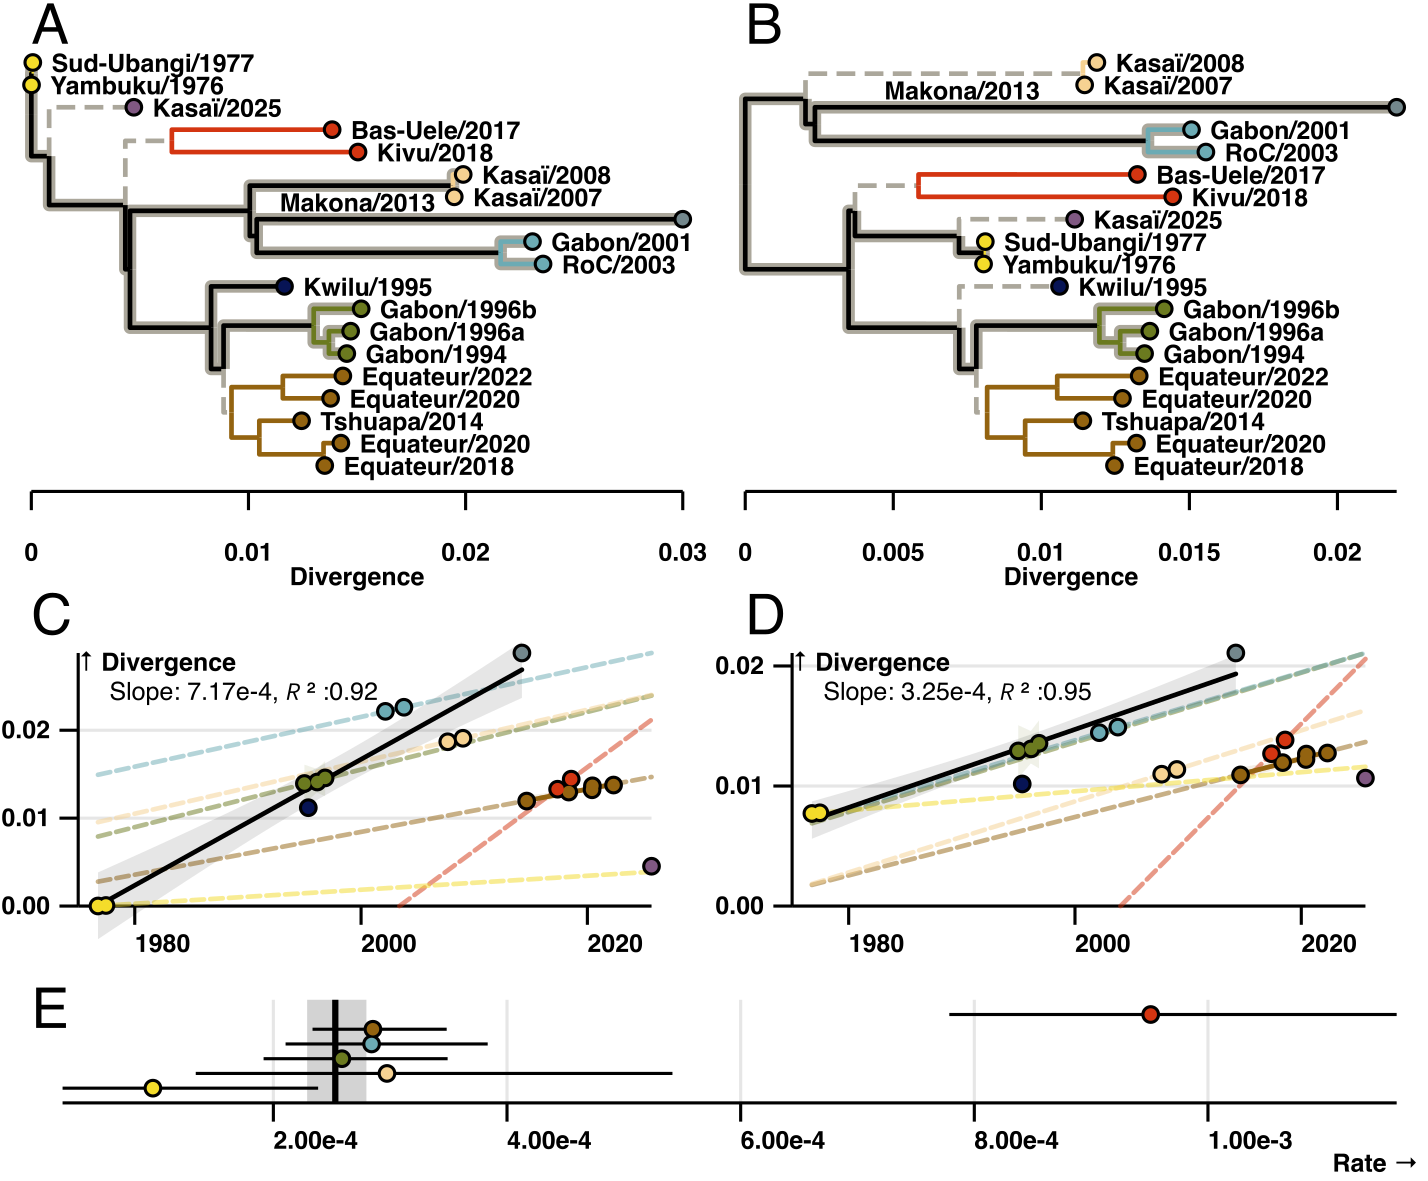
\includegraphics[width=1\textwidth]{figures/rtt.png} 
    \caption{Root-to-tip exploration of rate heterogeneity in the EBOV phylogeny. 
    A \& C) The EBOV phylogeny rooted at the accepted 1970s outbreak position and corresponding root-to-tip divergence plot. 
    B \& D) Similar to A and C but with the proposed rooting. 
    In all figures tips are coloured by outbreak cluster (Supplemental Figure~\ref{fig:map}A) and labelled by outbreak name (Supplemental Table~\ref{tab:genomes}).
    Branches in A and B that are highlighted in grey connect tips used in the full regressions in C and D. 
    Dashed, coloured regression lines are calculated for each cluster independently.
    E) The maximum-likelihood evolutionary rate estimated for each cluster independently. Bars represent the 95\% confidence interval (CI).
    The black vertical line represents the evolutionary rate estimated when all clusters share the same rate, with a grey box representing the 95\% CI.}
    \label{fig:rtt}
\end{figure*}

We estimated an independent evolutionary rate for each cluster in Figure~\ref{fig:rtt} using maximum likelihood and found remarkably similar rates across many clades (Figure~\ref{fig:rtt}E).
Interestingly, this analyses suggested EBOV evolves slower within these clades (2.53$ \times 10^{-4}$) than expected given the accepted root-to-tip correlation. 
The clade representing the 2017 and 2018 Northern DRC outbreaks (Bas-Uele/2017 and Kivu/2018) may exhibit a higher rate of evolution.
While this is consistent with previous results \cite{Mbala-Kingebeni2019-bo}, we note that this clade is characterised by long external branches which corresponds to a high variance in the estimated rate.

We hypothesized that if the within-cluster evolutionary rate represents EBOV evolution in the reservoir then there should be a root position that allows for similar between-cluster dynamics.
There is no rooting that does not require root-to-tip outliers with less divergence than their date would suggest.
However, if we root the EBOV phylogeny as in Figure~\ref{fig:rtt}B, there is a subset of branches that pass through the root, connect several outbreak clusters, and imply a similar between- and within- cluster evolutionary rate.

\begin{table*}[t]
\centering

    \begin{tabular}{lcrrrrrc}
    Data set & Model & LL & $\Delta$LL & df & p & Base rate & Root  \\ 
\toprule
Temporal set & DR & $−29893.4$ & $- $ & $- $ & $-$ & $-$ & $-$ \\ 
8 taxa & SRDT & $−29898.0$ & $−4.6 $ & $5 $ & 0.15 & 3.10$ \times 10^{-4}$ & Proposed \\ 
  & SRDT & $−29900.3$ & $−6.9 $ & $5 $ & 0.02 & 1.96$ \times 10^{-4}$ & Midpoint \\ 
  & SRDT & $−29906.6$ & $−13.2 $ & $5 $ & $<0.001$ & 7.56$ \times 10^{-4}$ & 1970s \\ 
  & SR & $−29915.6$ & $−22.2 $ & $6 $ & $<0.001$ & $-$ & Midpoint \\ 
  & SR & $−29931.2$ & $−37.9 $ & $6 $ & $<0.001$ & $-$ & Proposed \\ 
  & SR & $−30036.9$ & $−143.5 $ & $6 $ & $<0.001$ & $-$ & 1970s \\ 
\midrule
Classic temporal set & DR & $−31462.5$ & $- $ & $- $ & $-$ & $-$ & $-$ \\ 
11 taxa + Local clocks & localSRDT & $−31466.6$ & $−4.1 $ & $6 $ & 0.32 & 3.05$ \times 10^{-4}$ & Proposed \\ 
  & localSRDT & $−31469.8$ & $−7.4 $ & $6 $ & 0.02 & 2.02$ \times 10^{-4}$ & Midpoint \\ 
  & localSR & $−31487.9$ & $−25.5 $ & $7 $ & $<0.001$ & $-$ & Midpoint \\ 
  & SRDT & $−31503.0$ & $−40.6 $ & $8 $ & $<0.001$ & 6.89$ \times 10^{-4}$ & 1970s \\ 
  & localSR & $−31504.0$ & $−41.6 $ & $7 $ & $<0.001$ & $-$ & Proposed \\ 
  & SR & $−31634.6$ & $−172.2 $ & $9 $ & $<0.001$ & $-$ & 1970s \\ 
\midrule
Full data set & DR & $−34246.8$ & $- $ & $- $ & $-$ & $-$ & $-$ \\ 
19 taxa + Local clocks & localSRDT & $−34251.0$ & $−4.2 $ & $11 $ & 0.76 & 3.02$ \times 10^{-4}$ & Proposed \\ 
  & localSRDT & $−34255.6$ & $−8.9 $ & $11 $ & 0.12 & 2.24$ \times 10^{-4}$ & Midpoint \\ 
  & localSR & $−34284.7$ & $−38.0 $ & $12 $ & $<0.001$ & $-$ & Midpoint \\ 
  & localSR & $−34298.9$ & $−52.1 $ & $12 $ & $<0.001$ & $-$ & Proposed \\ 
  & localSRDT & $−34299.3$ & $−52.6 $ & $13 $ & $<0.001$ & 6.02$ \times 10^{-4}$ & 1970s \\ 
  & localSR & $−34566.8$ & $−320.1 $ & $14 $ & $<0.001$ & $-$ & 1970s \\ 
\bottomrule
\end{tabular}
\caption{Results of a TipDate analysis \cite{Rambaut2000-ss} for temporal signal in the 8 outbreaks highlighted in Figure \ref{fig:rtt}B and subsequent partitions with local clocks placed on non-cluster branches subtending the remaining outbreak clusters. 
Model - the clock model used (DR: different rates, i.e. no clock; SR: single rate, i.e. unidentifiable clock; SRDT: single rate dated tips, i.e. identifiable clock; localSR/SRDT - an SR/SRDT model with local clocks on between cluster branches not highlighted in Figure \ref{fig:rtt}).
For the 1970s root branches that appear dashed in Figure~\ref{fig:rtt}A have local clocks. For all other roots dashed branches in Figure~\ref{fig:rtt}B are used.
LL - Log likelihood, $\Delta$LL - Log likelihood difference from the best model,
df - degrees of freedom in a chi-squared test, p - p-value of a chi-squared test, 
Base rate - the inferred evolutionary rate (where applicable),
Root - the root position used in the analysis (see Supplemental Figure~\ref{fig:map}B)}
\label{tab:paml8}
\end{table*}

We found statistical support for clock-like evolution with an identifiable rate in the subtree of eight outbreaks highlighted in Figure \ref{fig:rtt}B when rooted at this proposed root \cite{Rambaut2000-ss}.
The proposed root position had the highest log-likelihood of all tested rootings ("Proposed" in Table~\ref{tab:paml8}), but a temporal signal was also observed when the tree was midpoint rooted with the Makona/2013 outbreak as an outgroup. 
Interestingly, we found no evidence for clock-like evolution in this dataset with the accepted root position near the Yambuku/1976 outbreak. 
These signals were maintained in a dataset comprised of the 11 outbreaks between 1976-2013 ("Classic temporal set") as well as in the full dataset of 19 samples when local clocks were applied to branches subtending the remaining clades (dashed branches in Figure~\ref{fig:rtt}B; Table \ref{tab:paml8}).
Our findings suggest the accepted root position of EBOV is based on a misguided interpretation of root-to-tip correlations.
However, clock-like evolution with periodic rate heterogeneity remains a plausible explanation for EBOV evolutionary dynamics. 


\subsection*{A mechanistic rate model discovers novel evolutionary dynamics}

We sought to determine if our proposed model for EBOV evolution is consistent with latency in the reservoir population.
To this end, we developed a state-dependent evolutionary rate model in which lineages transition between latent and replicating states (see Materials and Methods).
When in the replicating state, substitutions accumulate across branches according to an underlying evolutionary rate; however, the rate is zero whilst in the latent state.
We constrain our model such that all nodes are in the replicating state.
External nodes represent sampled, active infections, and internal nodes represent bifurcation events - both processes require replication.
Because of this constraint, latency is less likely on branches that span short periods of time, such as those seen within outbreak clusters, and more likely on the longer branches that connect outbreaks. 

We initially focused on the 18 outbreaks identified in Central Africa, based on the assumption that these may be connected by a contiguous reservoir population that excludes the geographically distant 2013 West African outbreak. 
The root proposed above had the highest posterior support (70.0\%) of all root positions with the remaining support split between trees with the Gabon/2001 and RoC/2003 (blue) clade or the Kasa{\"i}/2007-Kasa{\"i}/2008 cade (peach) as outgroups (Figure~\ref{fig:scNmBEAST} and Supplemental Figure~\ref{fig:nMallRoots}).
This analysis resulted in a mean root age of \scLatencyNoMakona{rootAge_mean} (95\% HPD: [\scLatencyNoMakona{rootAge_hpd_min}, \scLatencyNoMakona{rootAge_hpd_max}]) which corresponded to a mean replicating evolutionary rate of  \scLatencyNoMakona{clockRate_mean} s/s/y (95\% HPD: [\scLatencyNoMakona{clockRate_hpd_min}, \scLatencyNoMakona{clockRate_hpd_max}]) consistent with the exploration above.
We find evidence for wide-spread latency with median of \scLatencyNoMakona{latentBranches_median} branches exhibiting at least one period of latency (95\% HPD: [\scLatencyNoMakona{latentBranches_hpd_min}, \scLatencyNoMakona{latentBranches_hpd_max}]) (Figure~\ref{fig:scNmBEAST}A).
The average duration of latency on a branch with at least one period of latency was was 21.7 years (median 20.6 years) (Figure ~\ref{fig:scNmBEAST}).  
The five branches observed to be outliers in the root-to-tip plots are the only branches with a greater than 50\% posterior probability of at least one latent period (Figure~\ref{fig:scNmBEAST}A).


Our analysis suggests all latent lineages were seeded prior to 1980.
These lineages persisted until the mid 1990s, when they sparked a second wave of diversification (Figure~\ref{fig:scNmBEAST}B).
Interestingly all zoonotic outbreaks observed after the year 2013 derive from once latent lineages (Figure~\ref{fig:scNmBEAST}A).

\begin{figure*}[!hbtp]
    \centering
    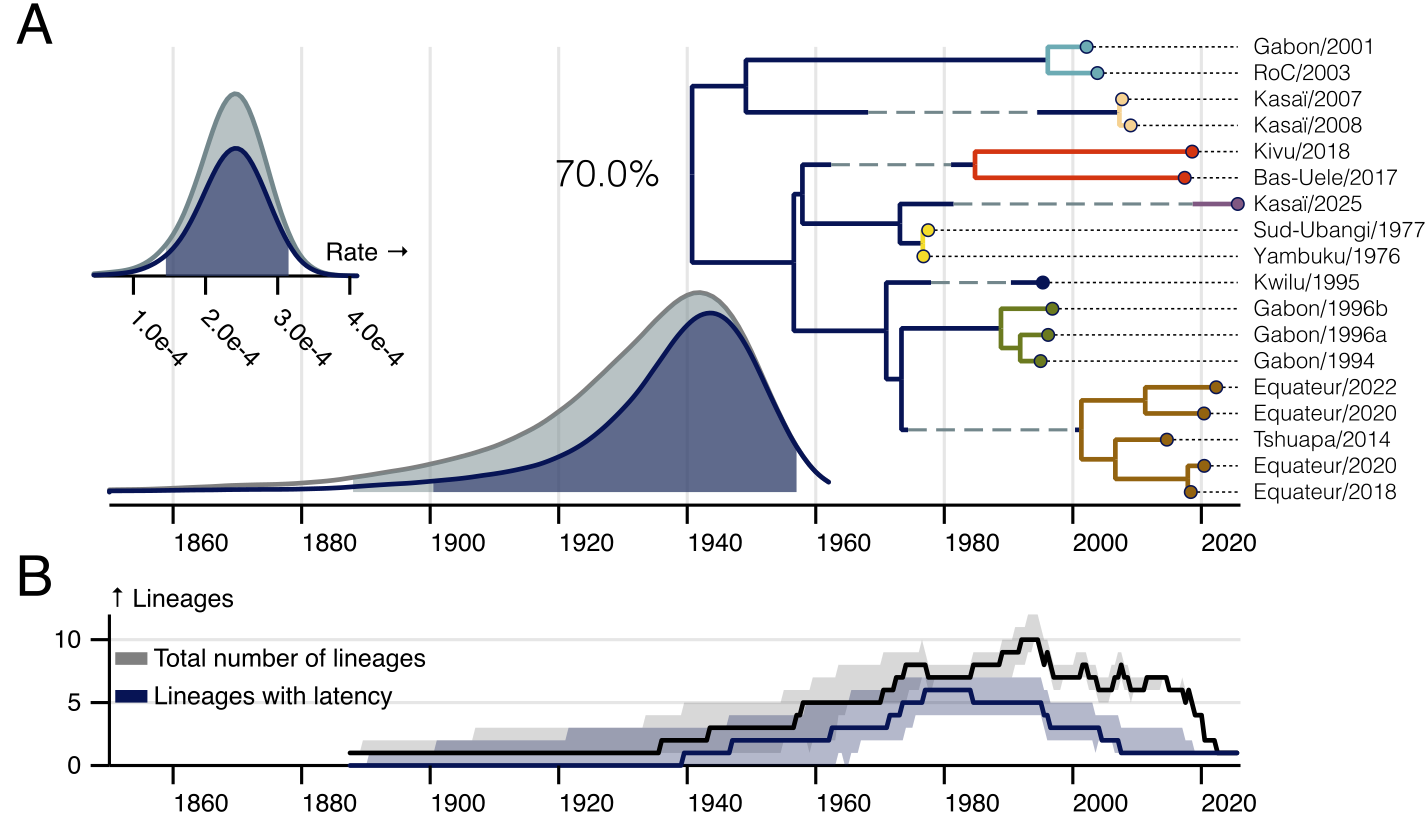
\includegraphics[width=1\textwidth]{figures/rootFigure.noMakona.png}
    \caption{Evolutionary history of EBOV in Central Africa.
    A) A maximum clade credibility (MCC) of tree of 18 EBOV outbreaks in Central Africa. 
    The tree summarises all trees with the displayed rooting.
    The posterior support for this rooting is displayed next to the root.
    Clades are coloured as in Figure~\ref{fig:rtt} with tips labelled by outbreak. The root age distribution of the entire analysis is shown in grey with the contribution of the displayed root highlighted in blue.
    For branches with greater than 50\% posterior support for latency, the posterior probability of latency is labelled above the branch. The mean duration of latency (conditioned on there being at least one period of latency) is shown as a dashed line centered between the parent and child node. 
    The marginal posterior root age distribution is shown in grey with contribution of the displayed root highlighted in blue.
    Inset: The posterior distribution of the evolutionary rate during replication, shaded by total analysis (grey) and conditioning on the displayed root (blue).
    In all posterior distribution plots, the shaded area represents the 95\% HPD.
    B) The number of lineages that exhibit latency through time. The median number of lineages that show any latency across the entire posterior is plotted as a solid line, with the 95\%HPD shown as a shaded area. 
    }
    \label{fig:scNmBEAST}
\end{figure*}


Despite being a geographic outlier, the 2013 West African outbreak is not a temporal outlier (Figure~\ref{fig:rtt}D).
Is a branch of this length consistent with our estimates of latency?
If we assume this outbreak diverges from the rest of EBOV near the root estimated above, its expected branch length would be \expectations{makona_mean} years long (95\% HPD [\expectations{makona_min}, \expectations{makona_max}]) which corresponds to a \expectations{makona_PL_mean} probability (\expectations{makona_PL_min}, \expectations{makona_PL_max}) of no latency.

Our findings were robust to the inclusion of this possible outlier, with the exception of increased uncertainty in the EBOV root placement. 
The mean root age of the extended dataset was \scLatency{rootAge_mean} (95\% HPD [\scLatency{rootAge_hpd_min}, \scLatency{rootAge_hpd_max}]) which corresponded to a similar replicating evolutionary rate of \scLatency{clockRate_mean} substitutions per site per year (95\% HPD: [\scLatency{clockRate_hpd_min}, \scLatency{clockRate_hpd_max}]).
Inclusion of the Makona/2013 outbreak resulted in a median of \scLatency{latentBranches_median} branches with latency (95\% HPD: [\scLatency{latentBranches_hpd_min}, \scLatency{latentBranches_hpd_max}]), with similar lineage through time dynamics (Figure~\ref{fig:scBEAST}C).

The underlying evolutionary rate is consistent with previous estimates, but we find less support for the proposed root position (16.9\% posterior support,Figure~\ref{fig:scBEAST}B).
Instead, the model favours a root with the Makona/2013 outbreak as an outgroup (33.7\%) (Figure~\ref{fig:scBEAST}A) .
The remaining posterior support was again split between trees with the Gabon/2001-RoC/2003 clade (blue) or the Kasa{\"i}/2007-Kasa{\"i}/2008 clade (peach) as outgroups  (Supplemental Figure~\ref{fig:allRoots}). 

\begin{figure*}[!hbtp]
    \centering
    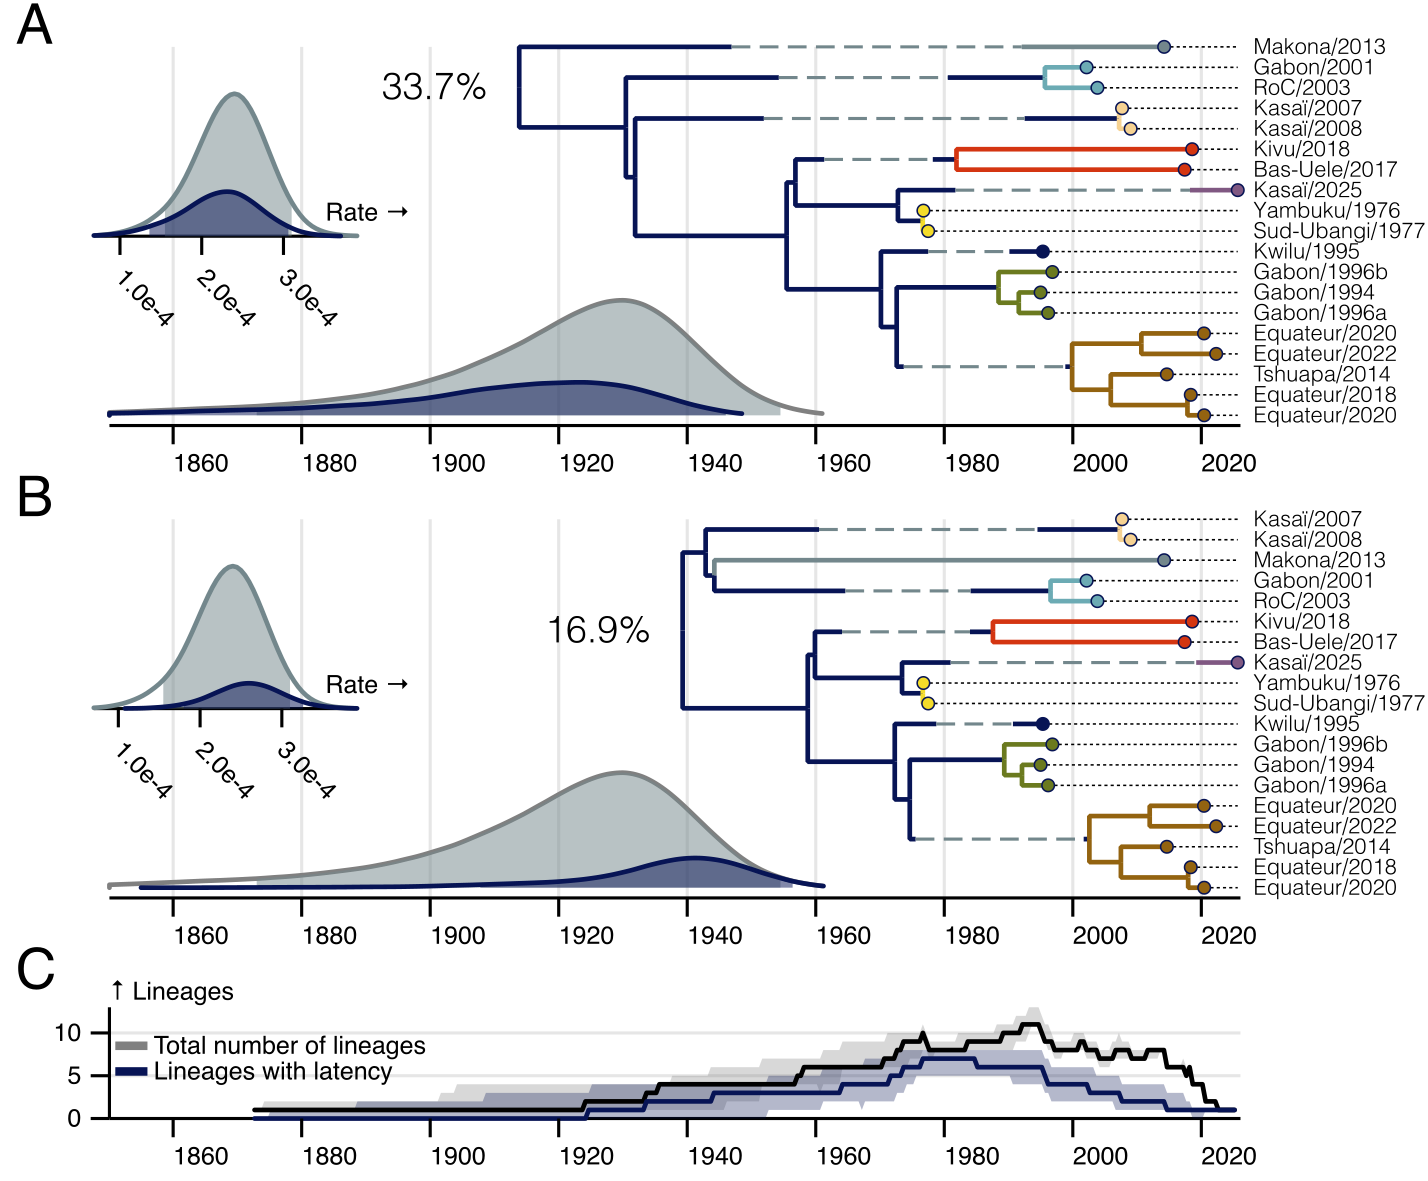
\includegraphics[width=1\textwidth]{figures/rootFigure.png}
    \caption{Posterior distributions of latency model parameters estimated for the full dataset partitioned by root position.
    A \& B) MCC trees of the most common root placement (A) and the proposed root (B) (posterior probability noted near root). 
    Clades are coloured as in Figure~\ref{fig:rtt} with tips labelled by outbreak. 
    The marginal posterior root age distribution is shown in grey with each root's conditional contribution is highlighted in blue.
    For branches with greater than 50\% posterior support for latency, the posterior probability of latency is labelled above the branch. The mean duration of latency (conditioned on there being at least one period of latency) is shown as a dashed line centred between the parent and child node. 
   Insets: The posterior distribution of the evolutionary rate during replication, again shaded by total analysis (grey) and conditioning on specific roots (blue).
    In all posterior distribution plots the shaded area represents the 95\% HPD. 
    C) The number of lineages that exhibit latency through time. The median of number of lineages that show any latency across the entire posterior is plotted as a solid line, with the 95\%HPD shown as a shaded area. }
    \label{fig:scBEAST}
\end{figure*}


\subsection*{The geographic spread of EBOV in Central Africa}

Previously, it was suggested that EBOV emerged from a genetic bottleneck near the Yambuku/1976 outbreak and then rapidly spread west through a wave-like process with a mean wave-front velocity of approximately 50 kilometers per year \cite{Walsh2005-zc}.
This estimated dispersal is a direct consequence of the root placement, and is inconsistent with our updated model.

We employed a continuous phylogeographic diffusion model with a single diffusion rate to characterize the geographic dispersal of EBOV alongside the latency model of EBOV evolution.
It has recently been show that more flexible phylogeographic approaches, which model diffusion as a branch-specific process are prone to misleading conclusions and overconfidence when applied to dynamic populations  \cite{Neher2025-ka}.
Although our model is likely over-simplified, it provides an interpretable starting point to explore the geographic implications of latency in the EBOV reservoir.

We found the EBOV root was located in western DRC near the 2014-2022 outbreaks in the Equateur province. 
This location is not unexpected given the nature of the phylogeographic diffusion modeled, and the topology of the tree, which is likely to place the root between geographically dispersed outbreak clusters (Figure~\ref{fig:scPhylogeo}A and \ref{fig:scPhylogeo}B).
Contrary to previous models, which found EBOV spread directionally from its root location, our model suggests EBOV dispersal was initially limited.
The location of most ancestral nodes matched that of the root (Figure~\ref{fig:scPhylogeo}B).

The location of the outbreak clusters and tree topology requires migrations from this ancestral source along three different axes (one northwesterly, one southerly, one northeasterly).
Interestingly, multiple independent lineages -- some latent -- follow each of these corridors. 
Similar geographic histories are not expected in independent clades of the tree in a purely diffusive process where location and genetic distance are highly correlated. 
These observations are robust to the inclusion of the West African outbreak which shifts the root location to the west and provides an addition migration along the northwestern axis (Supplemental Figure~\ref{fig:scPhylogeoFull}).
Together, these analyses suggest a geographic model in which EBOV circulation was constrained near the recent outbreaks in Equateur, DRC, followed by repeated disseminations along several migratory routes.


\begin{figure*}[!hbtp]
    \centering
    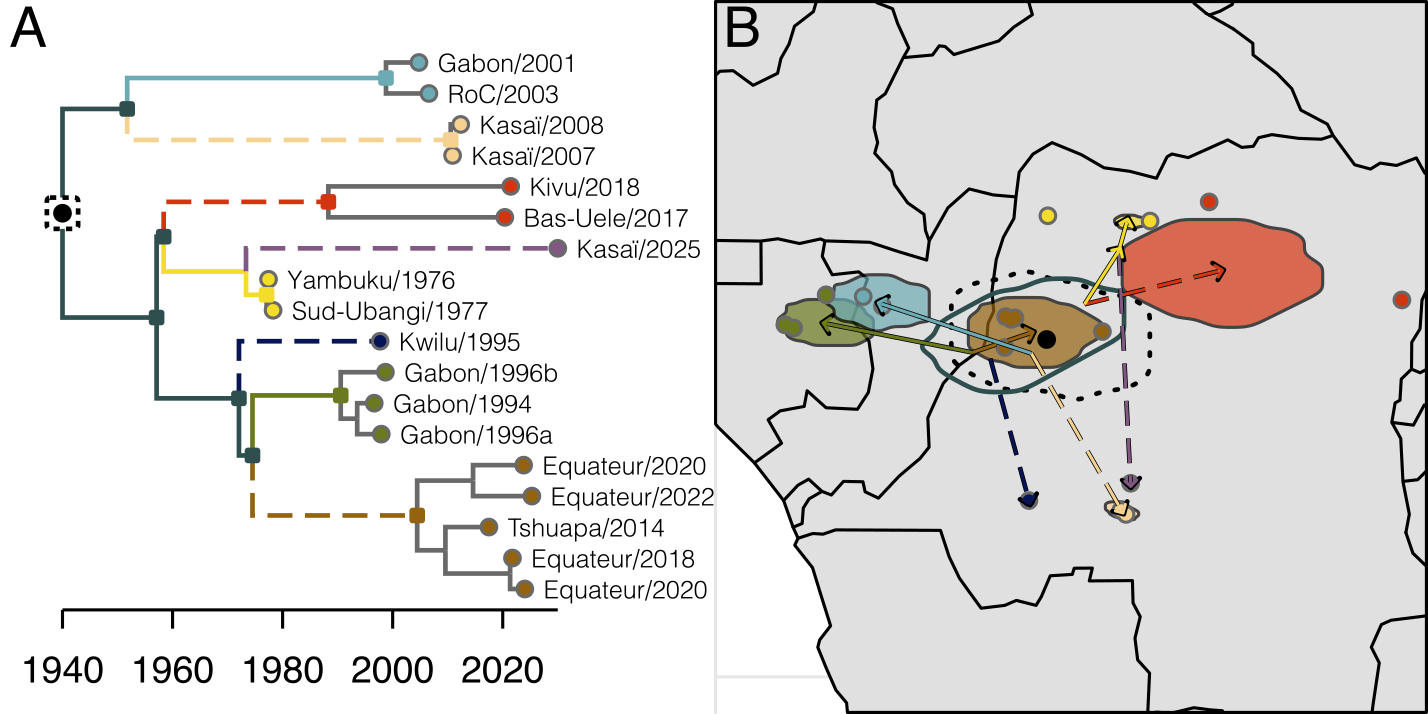
\includegraphics[width=1\textwidth]{figures/phyloGeo.png}
    \caption{The geographic implication of EBOV latency. 
    A) The MCC tree of the dataset when the West African outbreak is excluded. 
    Branches with more than 50\% posterior probability of at least one latent period are dashed, and those present in the map in B are coloured according to the clade they subtend.
    Tips are labelled by outbreak and coloured as previously.
    The root is denoted with a black circle surrounded by a dashed box, while ancestral nodes shown in B are highlighted with dark squares.
    B) A map depicting the geographic spread of EBOV. 
    The average root position is represented by a black circle.
    The 50\% HPD of the root position is enclosed by a dashed contour, while the 50\% HPD locations of the ancestral nodes (squares in A) is represented by the solid contour.
    The arrows represent the mean source and destination of the similarly coloured branches in A. 
    Outbreaks are shown as coloured circles, and the 50\% HPD of the MRCA of each outbreak clade is denoted as a shaded contour.
   }
    \label{fig:scPhylogeo}
\end{figure*}



\section*{Discussion}

An accurate model of EBOV evolution in the reservoir has important consequences for how we classify outbreaks and evaluate the risk of future epidemics. 
Decreased rates of evolution are thought to be a marker of human-derived outbreaks \cite{Garry2021-mw}.
In the initial phylogenetic analysis of the Equateur/2020 outbreak, one genome was found to cluster near the base of the Equateur/2018 outbreak \cite{Kinganda-Lusamaki2024-kg}.
The sample was thought to represent secondary transmission from a persistent human case.
However, there was no epidemiological evidence for this noted at the time, and this sequence's divergence is consistent with our modified estimate of EBOV's evolutionary rate (note the two Equateur/2020 isolates in Figure~\ref{fig:rtt}).
Given our updated model, this sample likely represents an independent spillover event from a large, diverse reservoir active in Equateur province, DRC, between 2018-2022, and not a persistent human case.

Given our finding that latency is wide-spread in EBOV evolution, it may be tempting to conclude that many EBOV outbreaks have resulted from persistently infected survivors of previous, unobserved outbreaks.
Perhaps humans make up a significant proportion of the reservoir.
We believe this to be implausible.
Persistence in humans -- although observed -- is exceedingly rare, and only associated with the largest epidemics. 
Such an EBOV reservoir would require large, unobserved human epidemics.
Additionally, our analysis identifies latency on several internal branches, precluding the possibility that these branches represent persistent human infections.


Our model suggests EBOV diversity predates the first observed outbreaks in the 1970s, and does not require EBOV to have emerged from a genetic bottleneck just prior to the first recorded human outbreak.
Although seemingly supported by the root-to-tip model at the time, this bottleneck and subsequent rapid expansion across the continent defied ready explanation from a disease ecology point of view.

Finally, we hypothesize that the phenomenon of EBOV persistence and latency in the reservoir is a mechanism by which the virus can maintain itself long term in a highly-structured host population - i.e., high-density but geographically dispersed bat roosts.
Younger bats dispersing to other colonies for mating, whilst persistently infected, may be the route of transmission between roosts.
Several of the migratory branches proposed by our phylogeographic model exhibit latency.
Furthermore, persistent infections within a roost may spark a new outbreak years later after sufficient immunologically-naïve individuals have been born.
This then establishes a new cohort of persistently infected individuals.
While similar models of persistence have been proposed \cite{Sundaram2025-gi,Plowright2016-ep}, such hypotheses have remained untested.
Here we have shown persistence combined with periods of latency is consistent with the phylogenetic patterns we observe between human outbreaks of EBOV.

The reservoir composition and dynamics of Ebola virus have evaded characterisation since the virus was first isolated in the late 1970s.
Our work here has used phylogenetic analyses to provide a sketch of the reservoir from its periodic spillover into humans.
Filling in the details, the mechanisms behind latency, and its implications for host dynamics are crucial to understanding when and where EBOV will emerge next.

\section*{Competing interests}
None declared.


\section*{Acknowledgments}
JTM, MAS and AR are grateful for support from the Wellcome Trust (Collaborators Award 206298/Z/17/Z, ARTIC network).
GB acknowledges support from the Research Foundation - Flanders (``Fonds voor Wetenschappelijk Onderzoek - Vlaanderen,'' G098321N), from the European Union Horizon 2023 RIA project LEAPS (grant agreement no. 101094685), and from the DURABLE EU4Health project 02/2023-01/2027, which is co-funded by the European Union (call EU4H-2021-PJ4) under Grant Agreement No. 101102733.
LMC was partly funded by FAPERJ - Fundação Carlos Chagas Filho de Amparo à Pesquisa do Estado do Rio de Janeiro, Processo SEI 260003/005679/2023 and SEI 260003/013252/2024.
GD acknowledges the support of European Molecular Biology Organization (EMBO) installation grant IG-5305-2023.
PM and AR acknowledge support from the Wellcome Trust (Discretionary Award 313694/Z/24/Z, ARTIC 2).
IFO thanks the Wellcome Trust Hosts, Pathogens \& Global Health program (Wellcome Trust, grant 218471/Z/19/Z) in partnership with Tackling Infectious Disease to Benefit Africa.
MAS and AR acknowledge support from National Institutes of Health (NIH) grant R01 AI153044 and the European Research Council (grant agreement no. 725422 -- ReservoirDOCS).
MAS acknowledges further support from NIH grants R01 AI162611 and R01 AI192139.

\pagebreak
\textbf{}

\printbibliography
\pagebreak


\section* {Supplemental information}

\beginsupplement



\section*{Supplemental Figures}

\begin{figure*}[!hbtp]
    \centering
    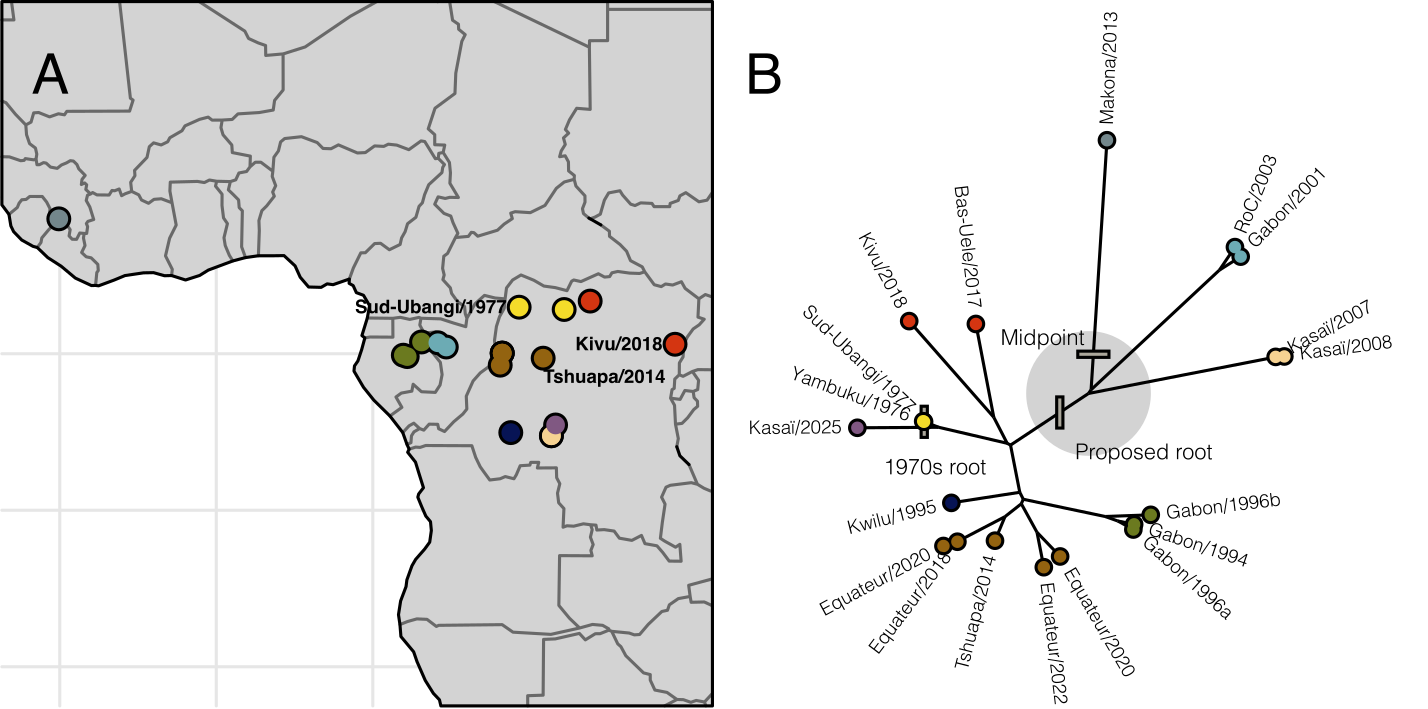
\includegraphics[width=1\textwidth]{figures/mapFigure.png}
    \caption{\textbf{A map (A) and unrooted tree (B) representing the outbreaks included in this study.} Common and proposed root placements are noted on the tree. The large grey sphere represents plausible root positions proposed by the latency rate model.}
    \label{fig:map}
\end{figure*}

\begin{figure*}[!hbtp]
    \centering
        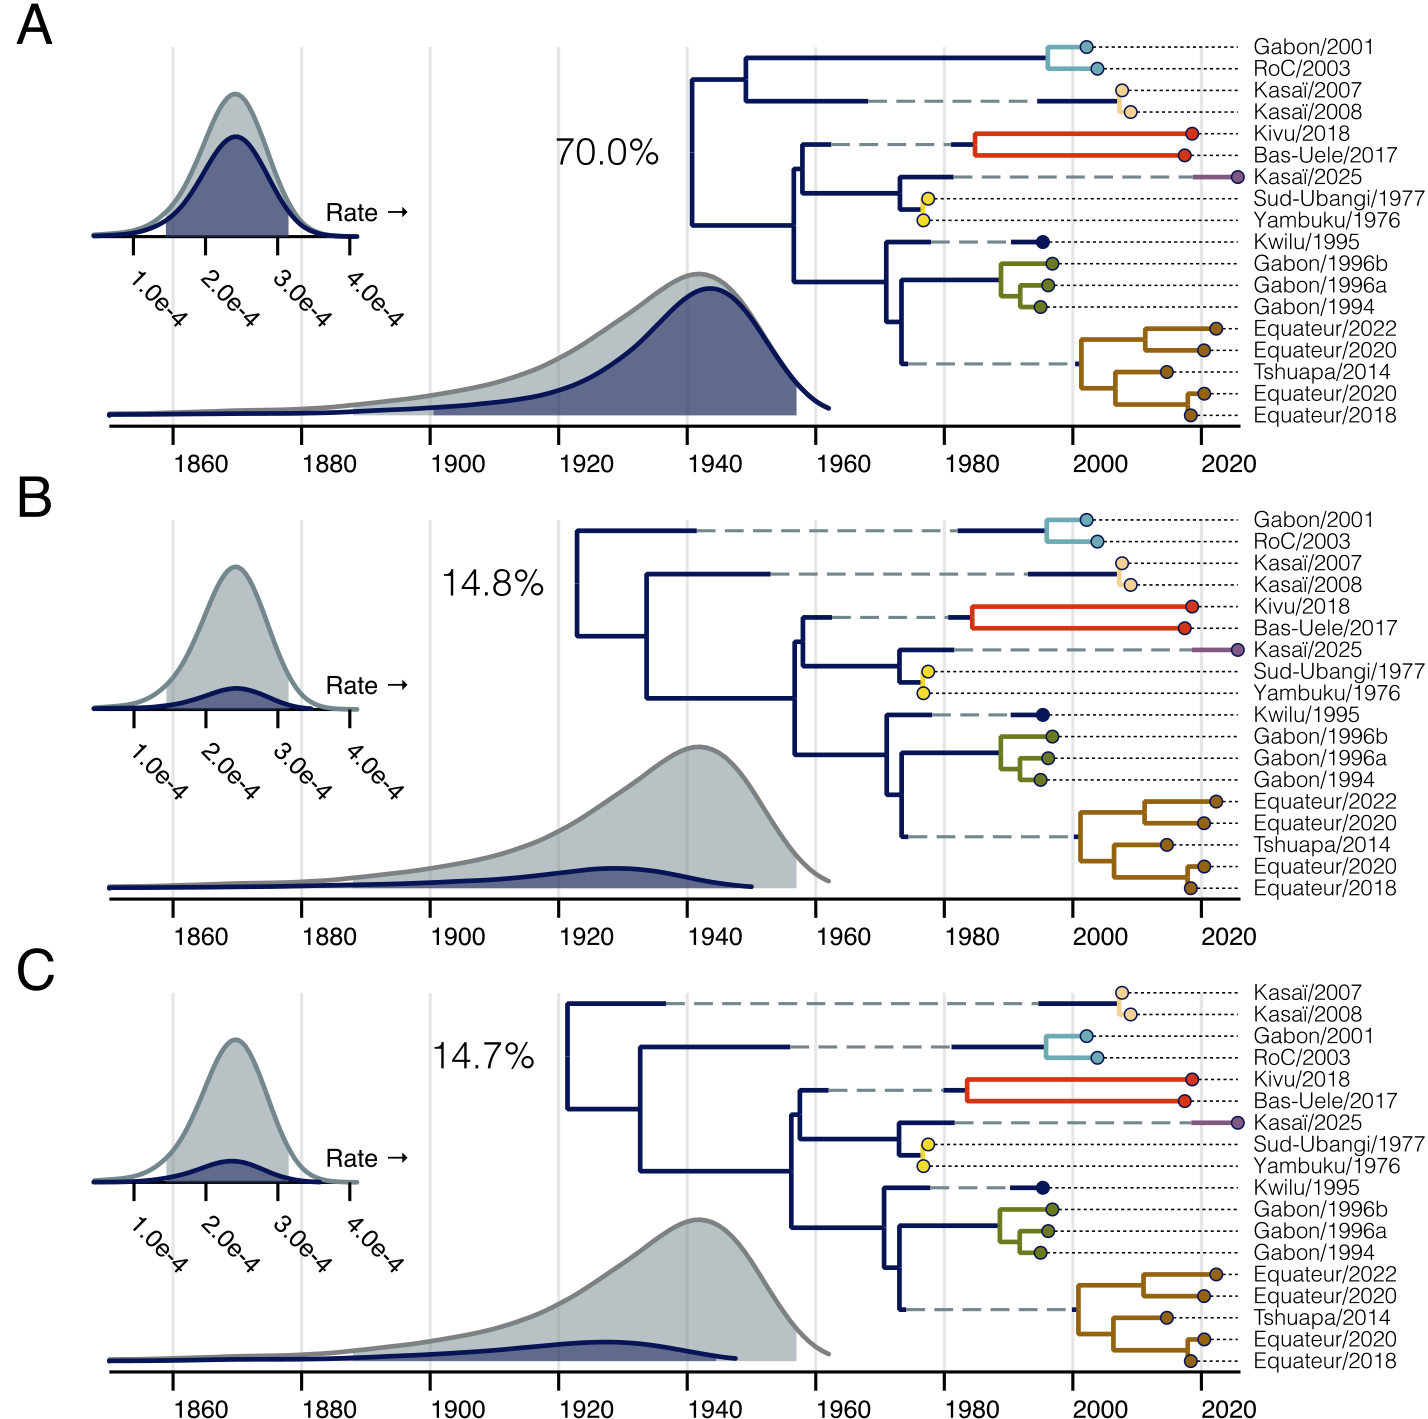
\includegraphics[width=1\textwidth]{figures/allRoots.noMakona.png}
   \caption{
     \textbf{The evolutionary history of EBOV in Central Africa under the latent model (all explored roots).} 
	Same as Figure~\ref{fig:scNmBEAST} but for all rootings with greater than 5\% posterior support.
   } 
    \label{fig:nMallRoots}
\end{figure*}

\begin{figure*}[!hbtp]
    \centering
        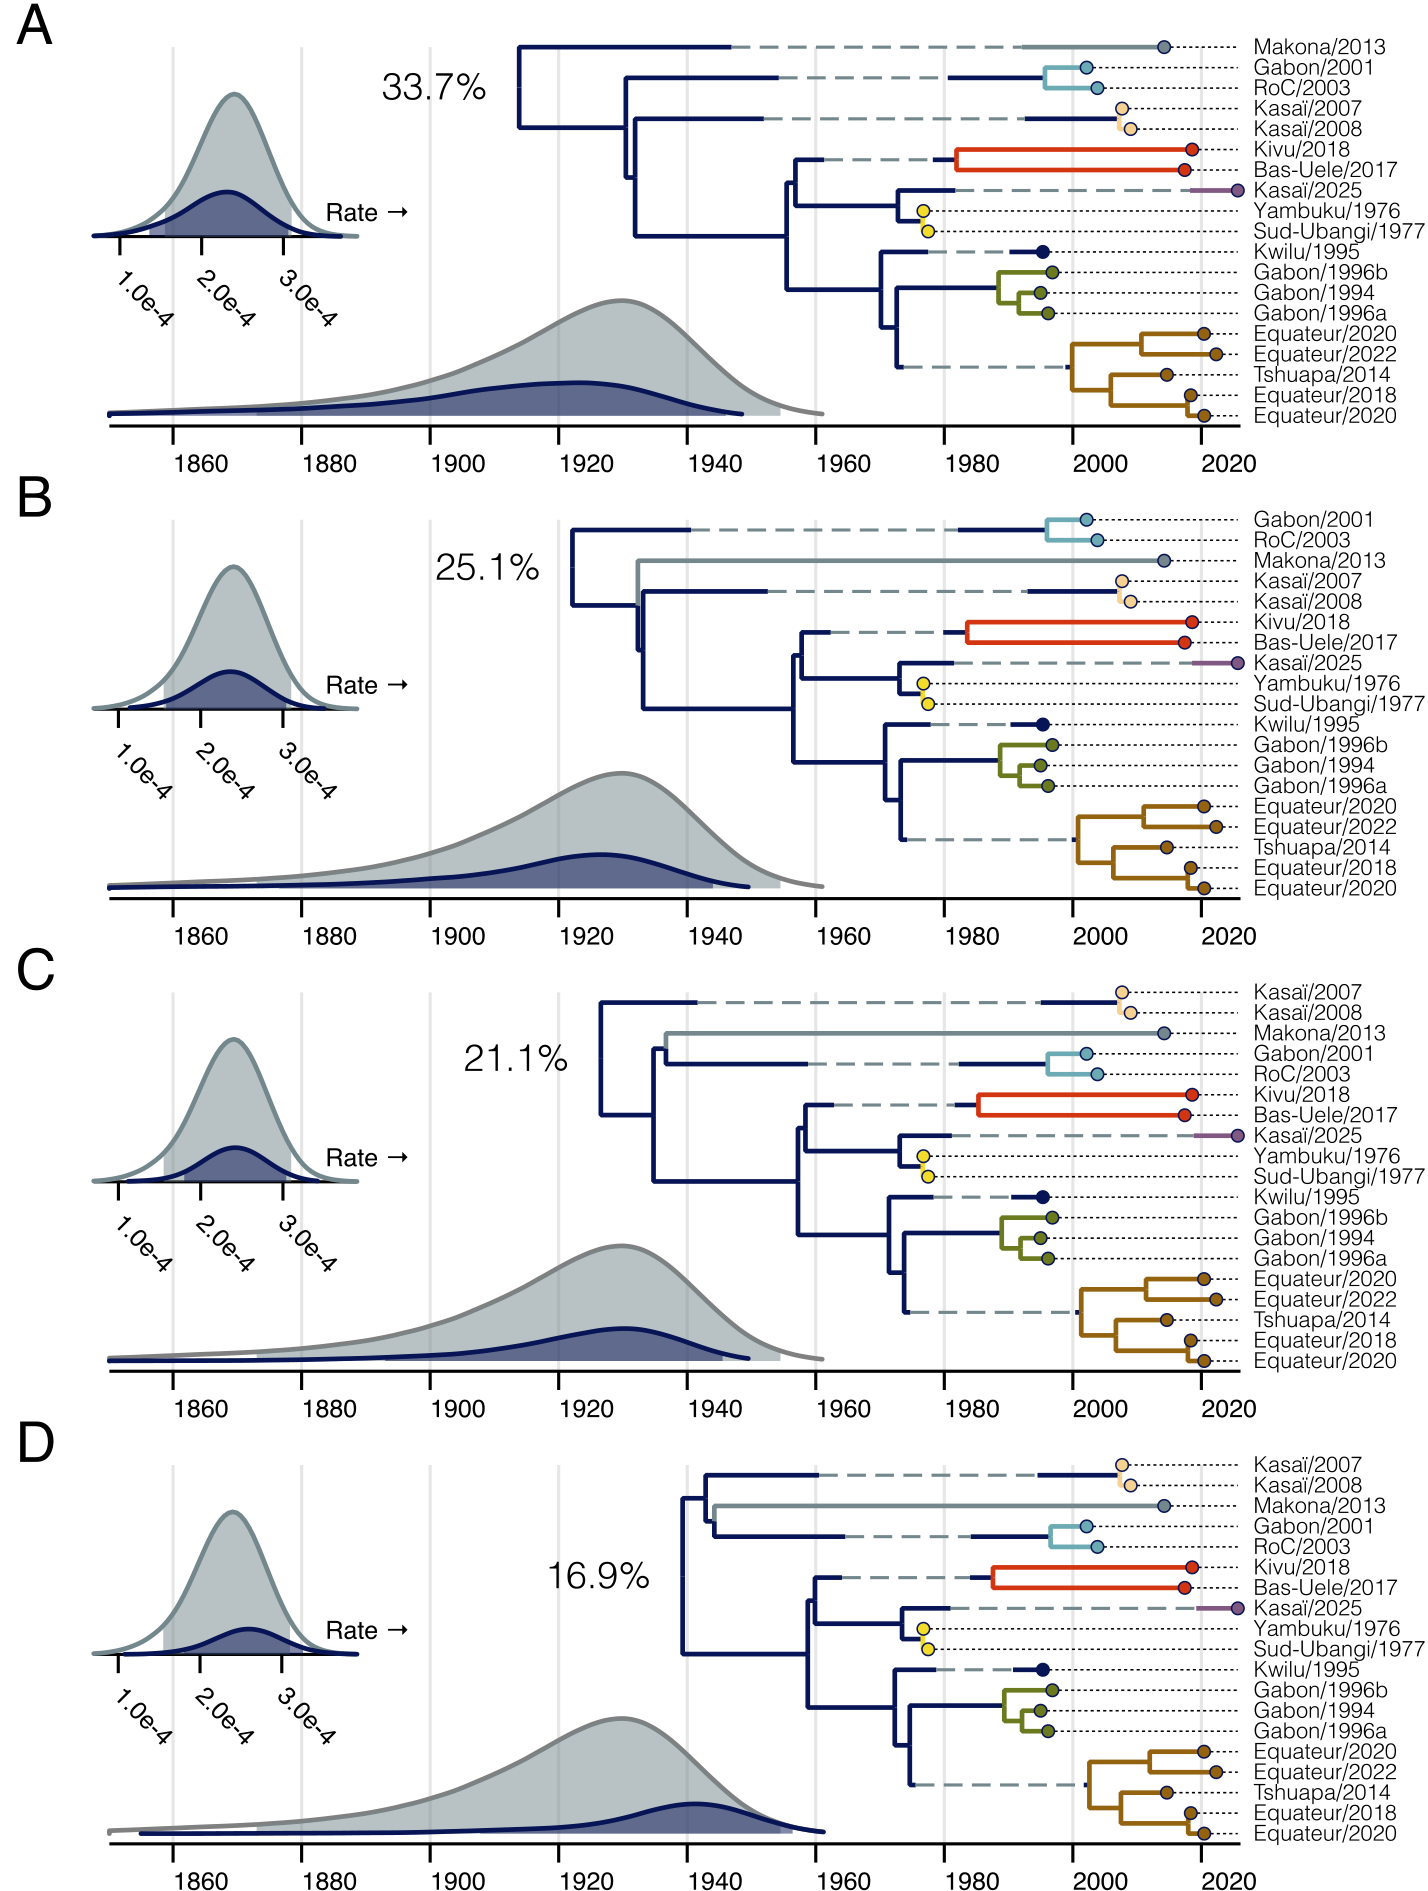
\includegraphics[width=1\textwidth]{figures/allRoots.png}
    \caption{\textbf{The evolutionary history of all EBOV outbreaks under the latent model partitioned by root position (all explored roots).} 
	Same as Figure~\ref{fig:scBEAST} but for all rootings with greater than 5\% posterior support.
   } 
    \label{fig:allRoots}
\end{figure*}

\begin{figure*}[!hbtp]
    \centering
    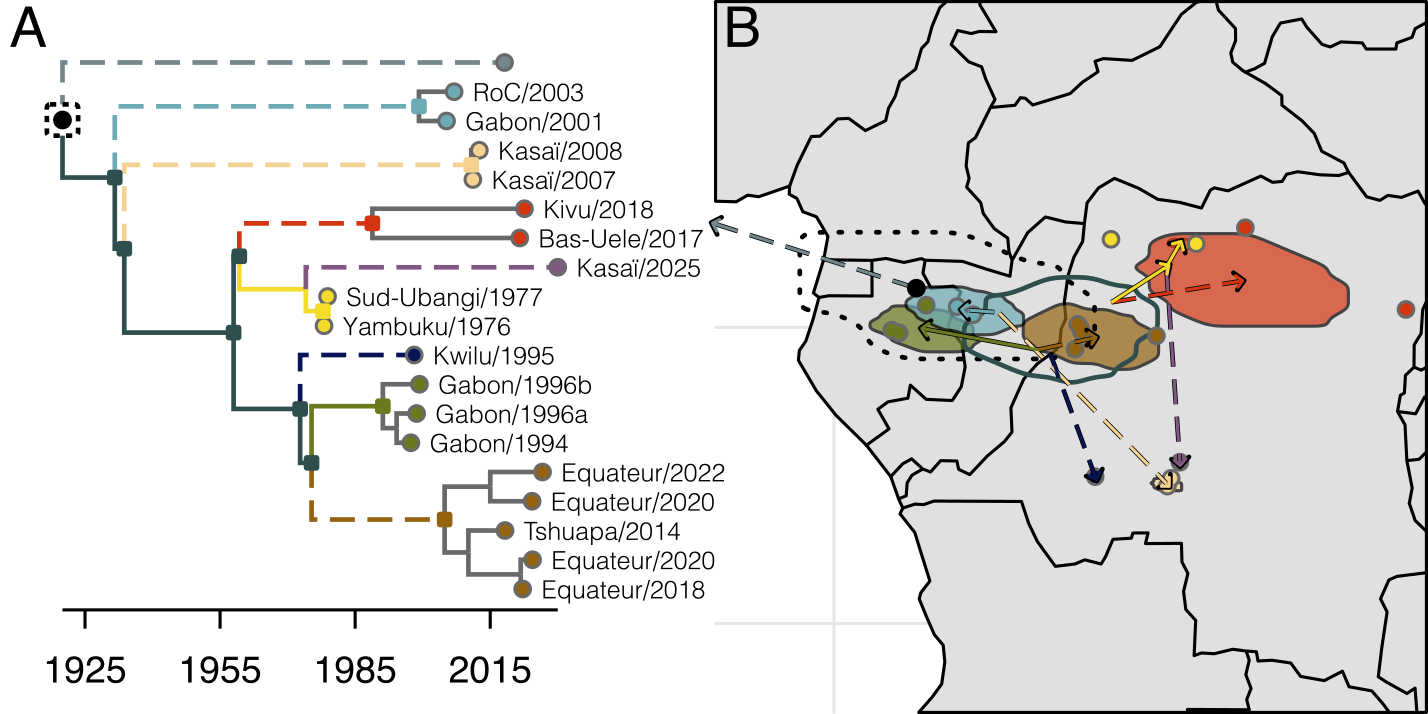
\includegraphics[width=1\textwidth]{figures/phyloGeo-full.png}
 \caption{\textbf{The geographic implication of latency in the EBOV reservoir including Makona/2013.} 
	Same as Figure~\ref{fig:scPhylogeo} but the Makona/2013 sample has been included in the analysis. 
   }
    \label{fig:scPhylogeoFull}
\end{figure*}

\begin{table}
    \centering
    \caption{\textbf{Recorded EBOV outbreaks used in this study.} Outbreak - the name of the outbreak; Country - the country of the outbreak; Adm1 - Administrative Region 1 of the outbreak. Duration - the dates of the outbreak. * indicates two genomes from the Equateur/2020 outbreak are present in our data.}
    
    \begin{tabular}{lllll}
Outbreak & Country  & Adm1  & Dates \\
\toprule
Yambuku/1976 & DRC & Mongala & Sep-Nov 1976 \\
Sud-Ubangi/1977 & DRC & Sud-Ubangi  & Jun-77 \\
Gabon/1994 & GAB & Ogooue-Ivindo & Dec 1994-Feb 1995 \\
Kwilu/1995 & DRC & Kwilu  & Jan-Jul 1995 \\
Gabon/1996a & GAB & Ogooue-Ivindo& Jan–Apr 1996 \\
Gabon/1996b & GAB & Ogooue-Ivindo  & Jul-96 \\
Gabon/2001 & GAB & Ogooue-Ivindo  & Oct 2001-Jul 2002 \\
% Mbomo-Kelle/2001 & COG & Cuvette Ouest & Lossi Animal Sanctuary & Dec 2001-May 2002 \\
% Mbomo-Kelle/2002 & COG & Cuvette Ouest & Kelle & Dec 2002–Apr 2003 \\
RoC/2003 & COG & Cuvette Ouest  & Oct-Dec 2003 \\
% Etoumbi/2005 & COG & Cuvette Ouest & Etoumbi & Apr-May 2005 \\
Kasaï/2007 & DRC & Kasai Occidental  & May-Nov 2007 \\
Kasaï/2008 & DRC & Kasai Occidental & Dec 2008–Feb 2009 \\
Makona/2013 & GIN & Gueckedou  & Dec 2013-Mar 2016 \\
Tshuapa/2014 & DRC & Tshuapa  & Aug–Nov 2014 \\
Bas-Uele/2017 & DRC & Bas Uele  & May-July 2017 \\
Equateur/2018 & DRC & Equateur & May-July 2018 \\
Kivu/2018 & DRC & Nord Kivu - Ituri - South Kiev & Aug 2018-June 2020 \\
Equateur/2020* & DRC & Equateur & June - Nov  2020 \\
Mbandaka/2022 & DRC & Equateur  & April- July 2022 \\
Kasaï/2025 & DRC & Kasai Occidental & August - October \\
\bottomrule
\end{tabular}
    \label{tab:oubtbreaks}
\end{table}

\begin{table}
\centering
\caption{\textbf{A list of the genomes used in this study with outbreak.} Accession refers to Pathoplexus accession and can be found at \cite{PP_SS_1057_2}. INSDC references the INSDC accesion for each sequence. Dataset denotes the smallest dataset in Table~\ref{tab:tipdater} which includes the taxa. Datasets build upon each other (e.g. the 11 taxa dataset adds 3 taxa to the 8 taxa dataset.)}

\begin{tabular}{llllll}
\toprule
Accession & INSDC & Country & Outbreak & Date & Dataset \\%& Authors\\
\toprule
PP\_000LS5R & KR063671 & DRC & Yambuku/1976 & 1976-10-01 & 8 taxa \\%&&\small{Das,S.R., Shabman,R., Halpin,R.A., Lin,X., Ransier,A., Fedorova,N., Tsitrin,T., Puri,V., Stockwell,T., Amedeo,P., Bishop,B., Gupta,N., Katzel,D., Schobel,S., Shrivastava,S., Alfson,K., Wentworth,D.E. and Griffiths,A.} \\
PP\_000LE61 & KC242791 & DRC & Sud-Ubangi/1977 & 1977-06 & 8 taxa \\%&&\small{Carroll,S.A., Towner,J.S., Sealy,T.K., McMullan,L.K., Khristova,M.L., Burt,F.J., Swanepoel,R., Rollin,P.E. and Nichol,S.T.}\\
PP\_000LE7Z & KC242792 & GAB & Gabon/1994 & 1994-12-27 & 8 taxa \\%&&\small{Carroll,S.A., Towner,J.S., Sealy,T.K., McMullan,L.K., Khristova,M.L., Burt,F.J., Swanepoel,R., Rollin,P.E. and Nichol,S.T.}\\
PP\_000MEGD & KU182905 & DRC & Kwilu/1995 & 1995-05-04 & 11 taxa \\%&&\small{Das,S.R., Shabman,R., Halpin,R.A., Akopov,A., Fedorova,N., Puri,V.,  Stockwell,T., Amedeo,P., Bishop,B., Katzel,D., Schobel,S., Shrivastava,S., Brasel,T., Yun,N., Paessler,S., Dowling,W. and Barrett,A. }\\
PP\_000LE8X & KC242793 & GAB & Gabon/1996a & 1996-02 & 8 taxa \\%&&\small{Carroll,S.A., Towner,J.S., Sealy,T.K., McMullan,L.K., Khristova,M.L., Burt,F.J., Swanepoel,R., Rollin,P.E. and Nichol,S.T. }\\
PP\_000LEGF & KC242798 & GAB & Gabon/1996b & 1996-10-27 & 8 taxa \\%&&\small{Carroll,S.A., Towner,J.S., Sealy,T.K., McMullan,L.K., Khristova,M.L., Burt,F.J., Swanepoel,R., Rollin,P.E. and Nichol,S.T. }\\
PP\_000LEJA & KC242800 & GAB & Gabon/2001 & 2002-02-23 & 8 taxa \\%&&\small{Carroll,S.A., Towner,J.S., Sealy,T.K., McMullan,L.K., Khristova,M.L., Burt,F.J., Swanepoel,R., Rollin,P.E. and Nichol,S.T. }\\
PP\_000LEQY & KF113529 & COG & RoC/2003 & 2003-10 & 8 taxa \\%&&\small{Chiu,C.Y., Naccache,S.N., Fair,J.N., Schneider,B.S. and Grard,G.} \\
PP\_000LDHD & HQ613403 & DRC & Kasaï/2007 & 2007-08-31 & 11 taxa \\%&&\small{ Grard,G., Biek,R., Muyembe-Tamfum,J.-J., Formenty,P., Paweska,J. and Leroy,E.} \\
PP\_000LDGG & HQ613402 & DRC & Kasaï/2008 & 2008-12-31 & 11 taxa \\%&&\small{ Grard,G., Biek,R., Muyembe-Tamfum,J.-J., Formenty,P., Paweska,J. and Leroy,E.}\\
PP\_000LETS & KJ660347 & GIN & Makona/2013 & 2014-03-20 & 8 taxa \\%&&\small{Baize,S., Pannetier,D., Oestereich,L., Rieger,T., Koivogui,L., Magassouba,N., Soropogui,B., Sow,M.S., Keita,S., De Clerck,H., Tiffany,A., Dominguez,G., Loua,M., Traore,A., Kolie,M., Malano,E.R., Heleze,E., Bocquin,A., Mely,S., Raoul,H., Caro,V., Cadar,D., Gabriel,M., Pahlmann,M., Tappe,D., Schmidt-Chanasit,J., Impouma,B., Diallo,A.K., Formenty,P., Van Herp,M. and Gunther,S.} \\
PP\_000LN4X & KP271018 & DRC & Tshuapa/2014 & 2014-08-20 & 19 taxa \\%&&\small{Naccache,S.N., Mbala,P., Ngay,I., Makuwa,M., Mulembakani,P., Muyembe,J.J., Schneider,B.S. and Chiu,C.Y.}\\
PP\_000NR4Q & MH613311 & DRC & Bas-Uele/2017 & 2017-05-07 & 19 taxa \\%&&\small{ Nsio,J., Kapetshi,J., Makiala,S., Formenty,P., Raymond,F., Tshapenda,G., Boucher,N., Corbeil,J., Okitandjate,A., Mbuyi,G., Kiyele,M., Mondonge,V., Kikoo,M.J., Van Herp,M., Rollin,P., Barboza,P., Muyembe Muzinga,B., Kalenga,O.I., Ahuka,S., Fausther-Bovendo,H., Kebela Ilunga,B., Kobinger,G.P. and Muyembe,J.-J.T. }\\
PP\_000NR9E & MH733477 & DRC & Equateur/2018 & 2018-05-10 & 19 taxa \\%&&\small{Mbala,P., Pratt,C., Wiley,M.R., Makiala-Mandanda,S., Aziza,A., Di Paola,N., Diagne,M.M., Chitty,J.A., Diop,M., Ayouba,A., Vidal,N., Faye,O., Karhemere,S., Aruna,A., Nsio,J., Mulangu,F., Mukadi,D., Mukadi,P., Kombe,J., Mulumba,A., Duraffour,S., Likofata,J., Pukuta,E., Minogue,T., Sozhamannan,S., Gross,S., Schroth,G., Delaporte,E., Sanchez-Lockhart,M., Peeters,M., Muyembe,J.-J., Alpha Sall,A., Palacios,G. and Ahuka-Mundeke,S. }\\
PP\_000NRSD & MK007330 & DRC & Kivu/2018 & 2018-07-28 & 19 taxa \\%&&\small{ Mbala-Kingebeni,P., Aziza,A., Di Paola,N., Wiley,M.R., Makiala-Mandanda,S., Caviness,K., Pratt,C.B., Prieto,K., Chitty,J.A., Larson,P., Ayouba,A., Vidal,N., Karhemere,S., Diop,M., Diagne,M.M., Faye,M., Faye,O., Aruna,A., Nsio,J., Mulanga,F., Mukadi,D., Mukadi,P., Kombe,J., Mulumba,A., Duraffour,S., Likofata,J., Pukuta,E., Gonzalez,J., Bartlett,M.L., Sozhamannan,S., Gross,S., Schroth,G., Kuhn,J., Delaporte,E., Sanchez-Lockhart,M., Alpha Sall,A., Muyembe,J.-J., Peeters,M., Palacios,G. and Ahuka-Mundeke,S. }\\
PP\_000PJZ4 & OR084849 & DRC & Equateur/2020 & 2020-05-31 & 19 taxa \\%&&\small{ Kinganda-Lusamaki,E., Whitmer,S., Lokilo-Lofiko,E., Amuri-Aziza,A., Muyembe-Mawete,F., Makangara-Cigolo,J.C., Makaya,G., Mbuyi,F., Whitesell,A., Kallay,R., Choi,M., Pratt,C., Mukadi-Bamuleka,D., Kavunga-Membo,H., Matondo-Kuamfumu,M., Mambu-Mbika,F., Ekila-Ifinji,R., Shoemaker,T., Stewart,M., Eng,J., Rajan,A., Soke,G.N., Fonjungo,P.N., Otshudiema,J.O., Folefack,G.L.T., Pukuta-Simbu,E., Talundzic,E., Shedroff,E., Bokete,J.L., Legand,A., Formenty,P., Mores,C.N., Porzucek,A.J., Tritsch,S.R., Kombe,J., Tshapenda,G., Mulangu,F., Ayouba,A., Delaporte,E., Peeters,M., Wiley,M.R., Montgomery,J.M., Klena,J.D., Muyembe-Tamfum,J.-J., Ahuka-Mundeke,S. and Mbala-Kingebeni,P.}\\
PP\_000PJVC & OR084846 & DRC & Equateur/2020 & 2020-06-12 & 19 taxa \\%&&\small{Kinganda-Lusamaki,E., Whitmer,S., Lokilo-Lofiko,E., Amuri-Aziza,A., Muyembe-Mawete,F., Makangara-Cigolo,J.C., Makaya,G., Mbuyi,F., Whitesell,A., Kallay,R., Choi,M., Pratt,C., Mukadi-Bamuleka,D., Kavunga-Membo,H., Matondo-Kuamfumu,M., Mambu-Mbika,F., Ekila-Ifinji,R., Shoemaker,T., Stewart,M., Eng,J., Rajan,A., Soke,G.N., Fonjungo,P.N., Otshudiema,J.O., Folefack,G.L.T., Pukuta-Simbu,E., Talundzic,E., Shedroff,E., Bokete,J.L., Legand,A., Formenty,P., Mores,C.N., Porzucek,A.J., Tritsch,S.R., Kombe,J., Tshapenda,G., Mulangu,F., Ayouba,A., Delaporte,E., Peeters,M., Wiley,M.R., Montgomery,J.M., Klena,J.D., Muyembe-Tamfum,J.-J., Ahuka-Mundeke,S. and Mbala-Kingebeni,P. }\\
PP\_003V5NQ & - & DRC & Equateur/2022 & 2022-04-25 & 19 taxa \\%& &\small{Placide Mbala-Kingebeni, Jean-Jacques Muyembe, Steve Ahuka-Mundeke, Hugo Kavunga, Daniel Mukadi, Elisabeth Pukuta, Eddy Kinganda Lusamaki, Amuri Aziza, Jean Claude Makangara, Emmanuel Lokilo, Franck Edidi, Junior Bula Bula, Raphael Lumembe, Gabriel Kabamba, Fabrice Mambu, Joel Montgomery, Peter Fonjungo, Norbert Soke, Jacques Likofata, Vital Mondonge, Gervais Folefack, Prosper Djiguimde, John Otshudiema, Deby Mukendi, Dieudonné Mwamba, John Kombe, Sofonias Tessema, Didi Bofaka, Andrew Rambaut, Mike Wiley, Catherine Pratt}\\
PP\_003RXHG & - & DRC & Kasaï/2025 & 2025-09-01 & 19 taxa \\%&&\small{Adrienne Amuri-Aziza, Gradi Luakanda - Ndelemo, Jean-Claude Makangara-Cigolo, Prince Akil-Bandali, Princesse Paku-Tshambu, Sam Wilkinson, Louis Tshulo, Josh Quick, Andre Citenga, Chloe Muswamba-Kayembe, Olga Ntumba-Tshitenge, Emmanuel Lokilo-Lofiko, Fiston Cikaya-Kankolongo, Ola Rilia, Servet Kimbonza, Elisabeth Pukuta, Daniel Mukadi, Christian Ngandu, Mathias Mossoko, Gabriel Kabamba -Lungenyi, Raphael Lumembe-Numbi, Elzedeck Mabika-Bope, Patrick Mukadi, Catherine Pratt, Dieudonne Mwamba, Nick Loman, Andrew Rambaut, Eddy Kinganda-Lusamaki, Tony Wawina-Bokalanga, Dieudonne Mumba - Ngoyi, Jean-Jacques Muyembe-Tamfum, Steve Ahuka-Mundeke  Placide Mbala-Kingebeni }\\
\bottomrule
\end{tabular}
\label{tab:genomes}
\end{table}


\pagebreak

\section*{Supplemental text}



\subsubsection*{Further exploration of temporal signal}

The temporal outliers observed in the EBOV phylogeny could have resulted from enhanced purifying selection instead of latency.
To investigate this possibility, we repeated the analysis in Figure~\ref{fig:rtt} with a partition made of only third position codon sites and intergenic regions (Figure~\ref{fig:rtt-cds3_ig}).
Despite elevated evolutionary rates, which are expected for a dataset enriched in synonymous sites, this analysis produced the same conclusions as that run on the full genome.
Temporal outliers were maintained, as were our initial observations regarding within- and between-cluster rates. 

\begin{figure*}[!hbtp]
    \centering
    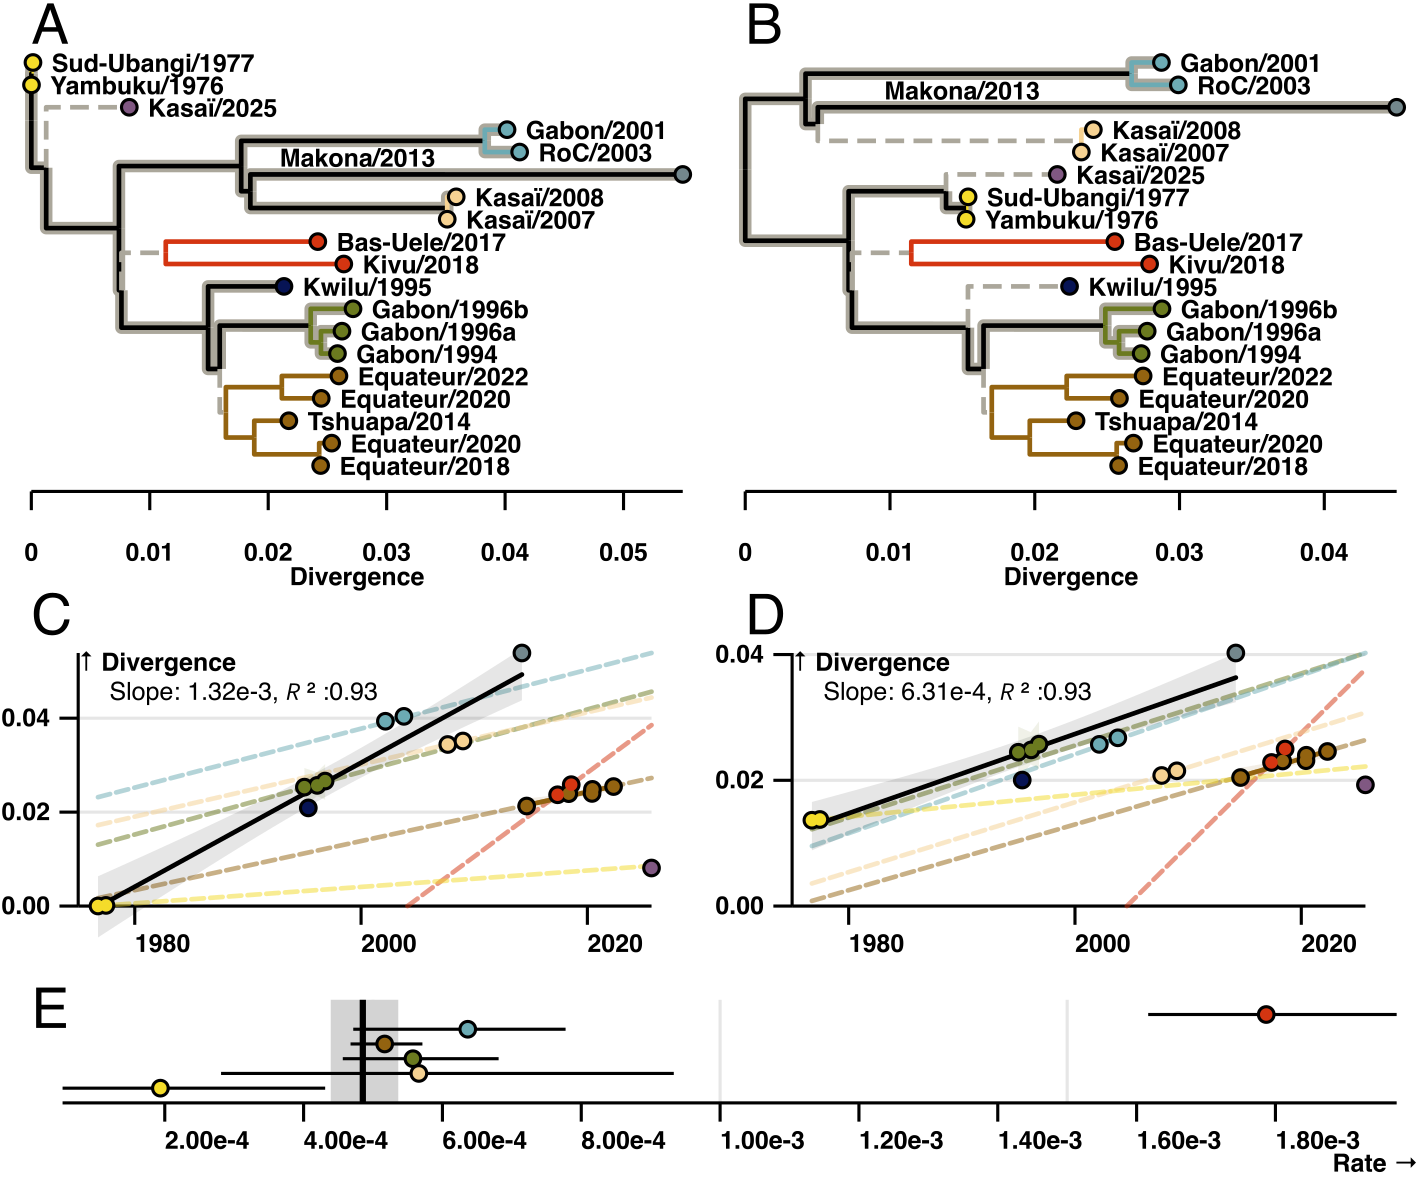
\includegraphics[width=0.8\textwidth]{figures/rtt-cds3_ig.png} 
     \caption{\textbf{Rate heterogeneity in the EBOV phylogeny (third position coding sites and intergenic regions).}
	Same as Figure~\ref{fig:rtt} with the exception that the presented phylogenies were made with only sites in the third codon position and intergenic regions.
	}    \label{fig:rtt-cds3_ig}
\end{figure*}


\subsection*{Prior sensitivity analysis}

Preliminary analyses suggested that when applied to the EBOV dataset the latency model is positioned between two extremes, both of which likely have identifiability issues.
If the rate of latent-replicating transition is too low relative to the scale of the tree, no latency is expected and the model reduces to a strict-clock model.
In this case, there is no temporal signal in the full dataset if a strick-clock model is employed.
The evolutionary rate is unidentifiable.

If the rate of transition is too high then the model approaches a free-rates model with an evolutionary rate on each branch. 
In some datasets where the parameters of the latency model may be known this could be tolerated.
However, our analyses show that we have little power to predict \emph{a priori} the amount of latency on a latent branch.
Note the wide spread in the distribution of time spent latent in Figure~\ref{fig:future}B. 

In this study we place a gamma prior on the rate of latent-replicating transitions.
The gamma distribution was parameterized with a rate parameter equal to the root height.
This prior was chosen to ensure the expected rate of latency scales with the phylogeny and strikes a balance between the extremes above without prohibiting either.
As noted in the methods, this prior favors no latency while still allowing for the possibility of latency (95\% prior probability of no latency).

We ran two additional analyses to explore the impact of this prior on our findings.
In the first, the rate of the gamma distribution was set to one half the root height, which would favor more latency (Figure~\ref{fig:nM-rh05}).
In the other, the rate of the gamma distribution was set to twice the root height, which favors less latency (Figure~\ref{fig:nM-rh2}).
Both analyses produced comparable results to that presented in the main text (Table \ref{tab:prior} and Figures~\ref{fig:nM-rh2} \& \ref{fig:nM-rh05}).
In fact, increasing the rate of the gamma prior by a factor of two increased the posterior support for the proposed root to nearly 90\% (Figures~\ref{fig:nM-rh2}).

\begin{table}[!hbp]
    \centering
    
\begin{tabular}{lrrr}
    Prior & Root age & Clock rate & Latent branches  \\ 
\toprule
Root height & 1929 [1887,1957]& 2.34$ \times 10^{-4}$ [1.41, 3.19] & 6 [5,9] \\
Root height $\div 2$ & 1924 [1878,1957] & 2.34$ \times 10^{-4}$ [1.42, 3.21] & 7 [5,11]\\
Root height $\times 2$ & 1934 [1903,1958] & 2.29$ \times 10^{-4}$ [1.36,3.08] & 6 [4,8] \\
\bottomrule
\end{tabular}
  \caption{\textbf{Prior sensitivity analysis.} Prior - the rate parameter of the gamma distribution placed on the latent rate. Root age- posterior mean and 95\% HPD of the root age. Clock rate- posterior mean and 95\% HPD of the evolutionary rate when replicating. Latent branches -  the median and 95\% HPD of the number of branches with at least one latent period.}
    \label{tab:prior}
\end{table}

\begin{figure*}[!hbtp]
    \centering
    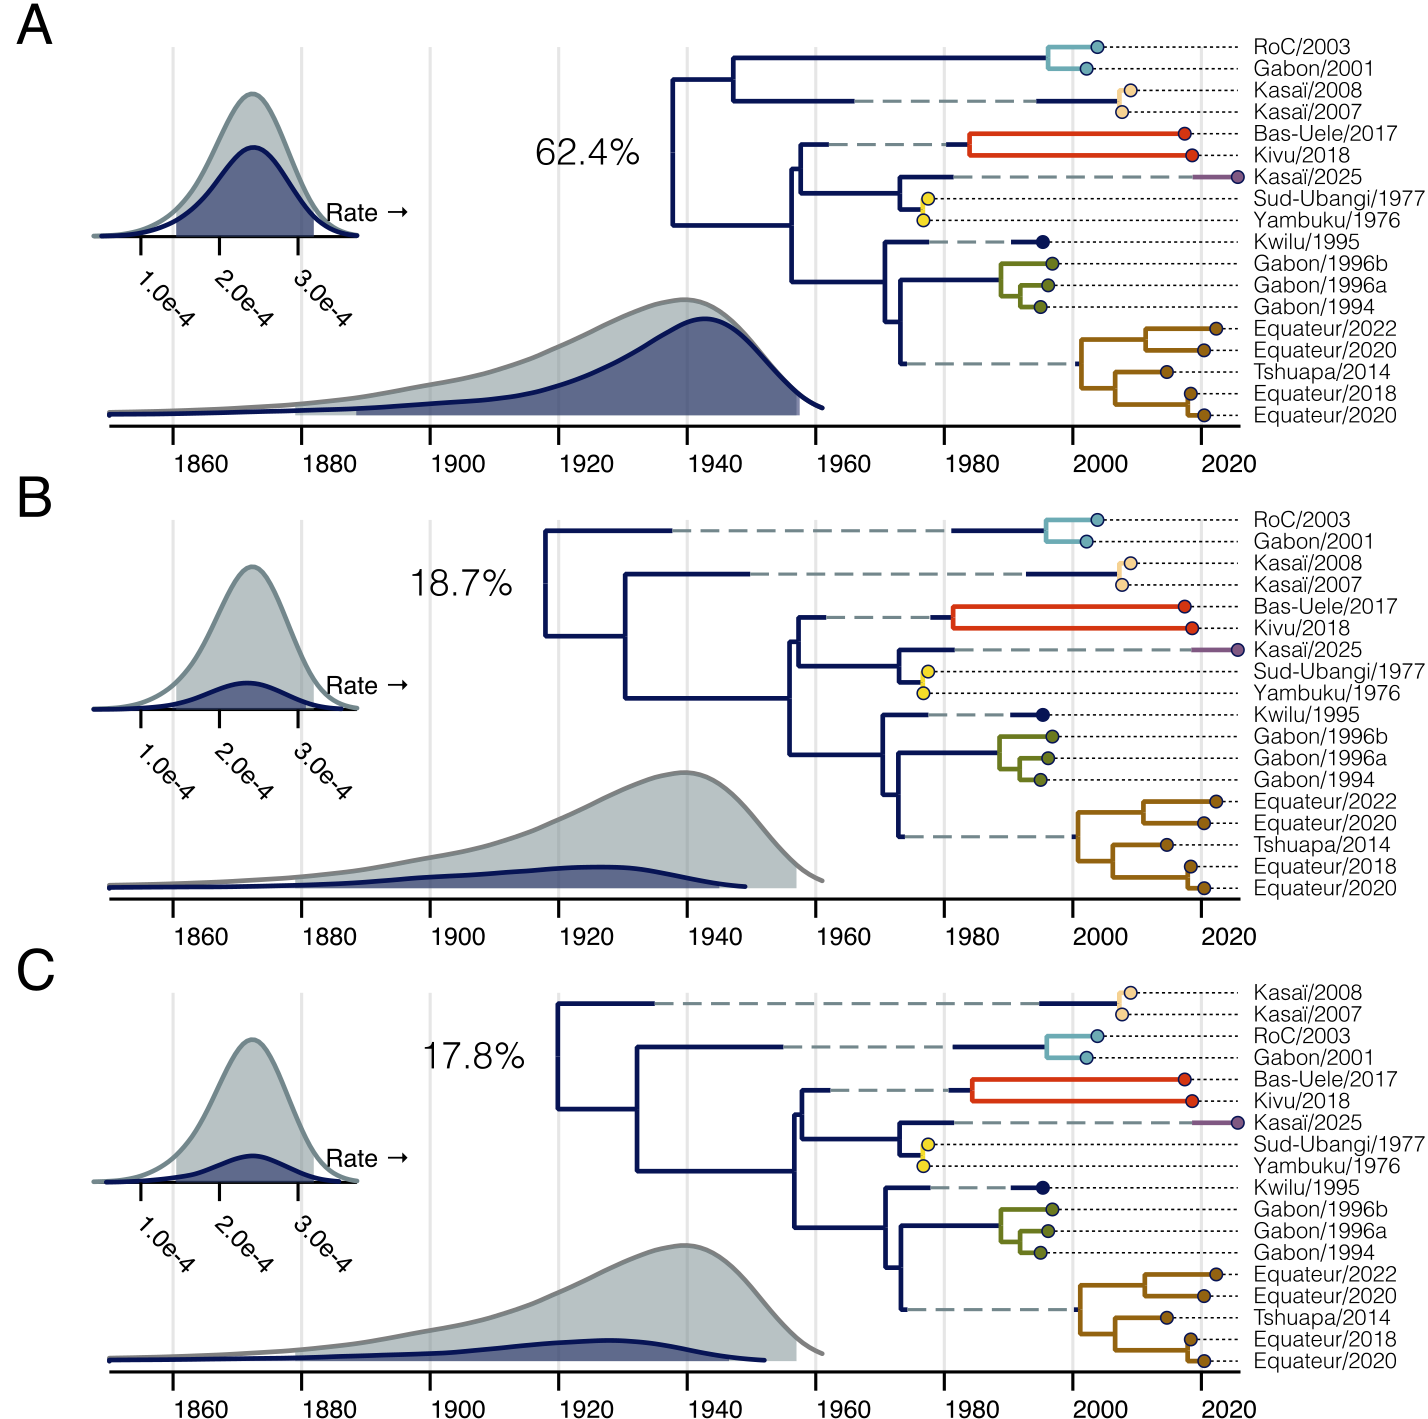
\includegraphics[width=1\textwidth]{figures/allRoots.noMakona-rh0.5.png}
  \caption{\textbf{Evolutionary history of EBOV in Central Africa with a prior favoring more latency.}
	Same as Figure~\ref{fig:nMallRoots}; however the rate parameter of gamma prior placed on the rate of latent transitions is one-half the root height.
    }
    \label{fig:nM-rh05}
\end{figure*}

\begin{figure*}[!hbtp]
    \centering
    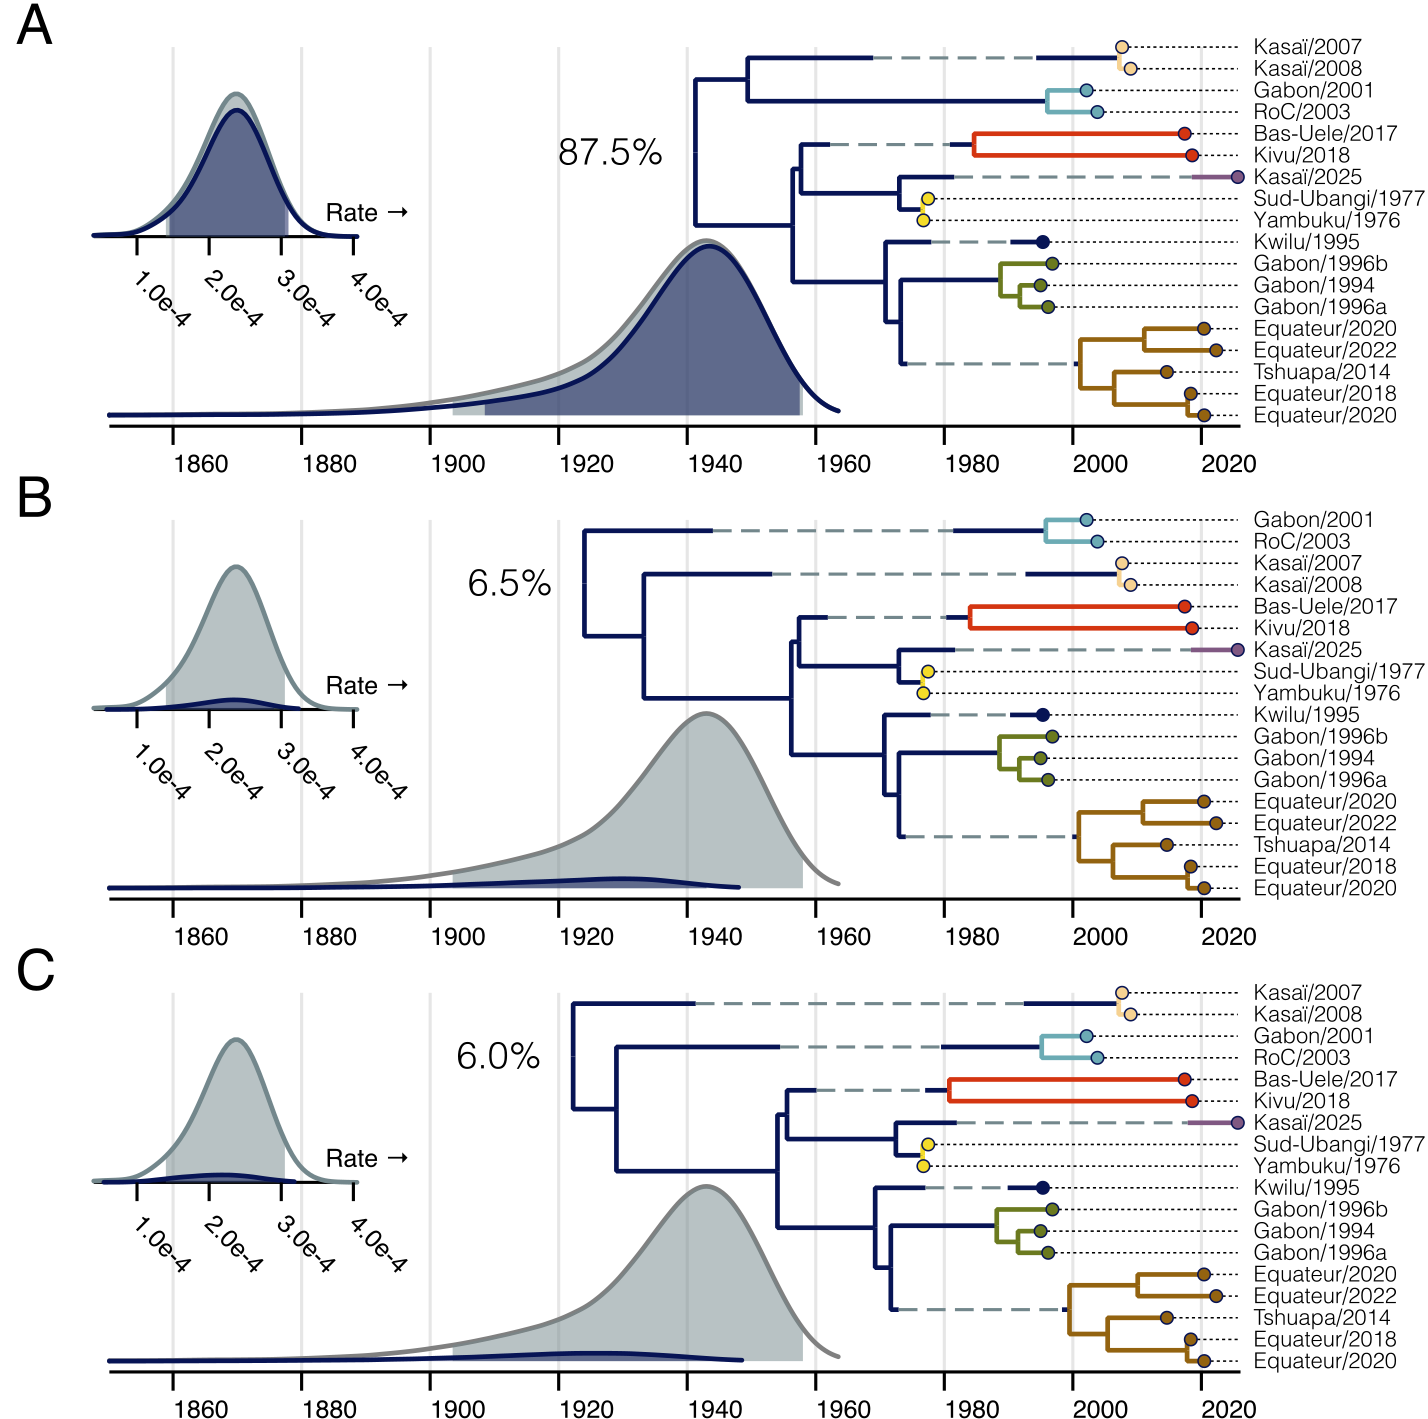
\includegraphics[width=1\textwidth]{figures/allRoots.noMakona-rh2.png}
    \caption{\textbf{Evolutionary history of EBOV in Central Africa with a prior favoring less latency.}
	Same as Figure~\ref{fig:nMallRoots}; however the rate parameter of gamma prior place the rate of latent transitions is twice the root height.
    }
    \label{fig:nM-rh2}
\end{figure*}


\end{document}

